\documentclass[12pt,a4paper]{article}
\usepackage[style = authoryear, maxcitenames = 1, uniquelist=false, sorting = nyt, abbreviate = true, doi = true, backend = biber]{biblatex}
\usepackage[lmargin = 3.5cm, rmargin = 3.5cm, tmargin = 2.5cm, bmargin = 2.5cm]{geometry}
\usepackage[onehalfspacing]{setspace}
\usepackage{graphicx}
\usepackage{hyperref}
\usepackage{times}
\usepackage{csquotes}
\usepackage[UKenglish]{babel}
\usepackage[textsize=tiny]{todonotes}
\usepackage[acronym]{glossaries}
\usepackage{soul} % for command \hl
\usepackage{pdfpages} % to insert pdf docs
\usepackage{csvsimple} % to import .csv files as tables
\usepackage{siunitx}
\usepackage{tikz}
\usepackage{caption} 
\usepackage{float}
\captionsetup[table]{skip=10pt} % more space between table and caption

\AtBeginBibliography{\small}
\addbibresource{main_sources.bib}

\setlength{\parindent}{0cm}
\setlength{\marginparwidth}{3.5cm} % make todonotes wider
\newcommand{\todoleft}[1]{{\reversemarginpar \todo{#1}}}
% preset for italic species name, abbreviated after first use
\newacronym[first = {\textit{Harmonia axyridis}}]{harm}{\textit{H. axyridis}}{\textit{Harmonia axyridis}}
\glsdisablehyper % no hyperref for \gls


%%%%%%%%%%%%%%%%%%%%%%%%%%%%%%%%%%%%%%%%%%%%%%%%%%%%%%%%%%%%%%%%%%
\begin{document}
\def\findate{16.05.2024}

%einreichung-der-bachelorarbeit
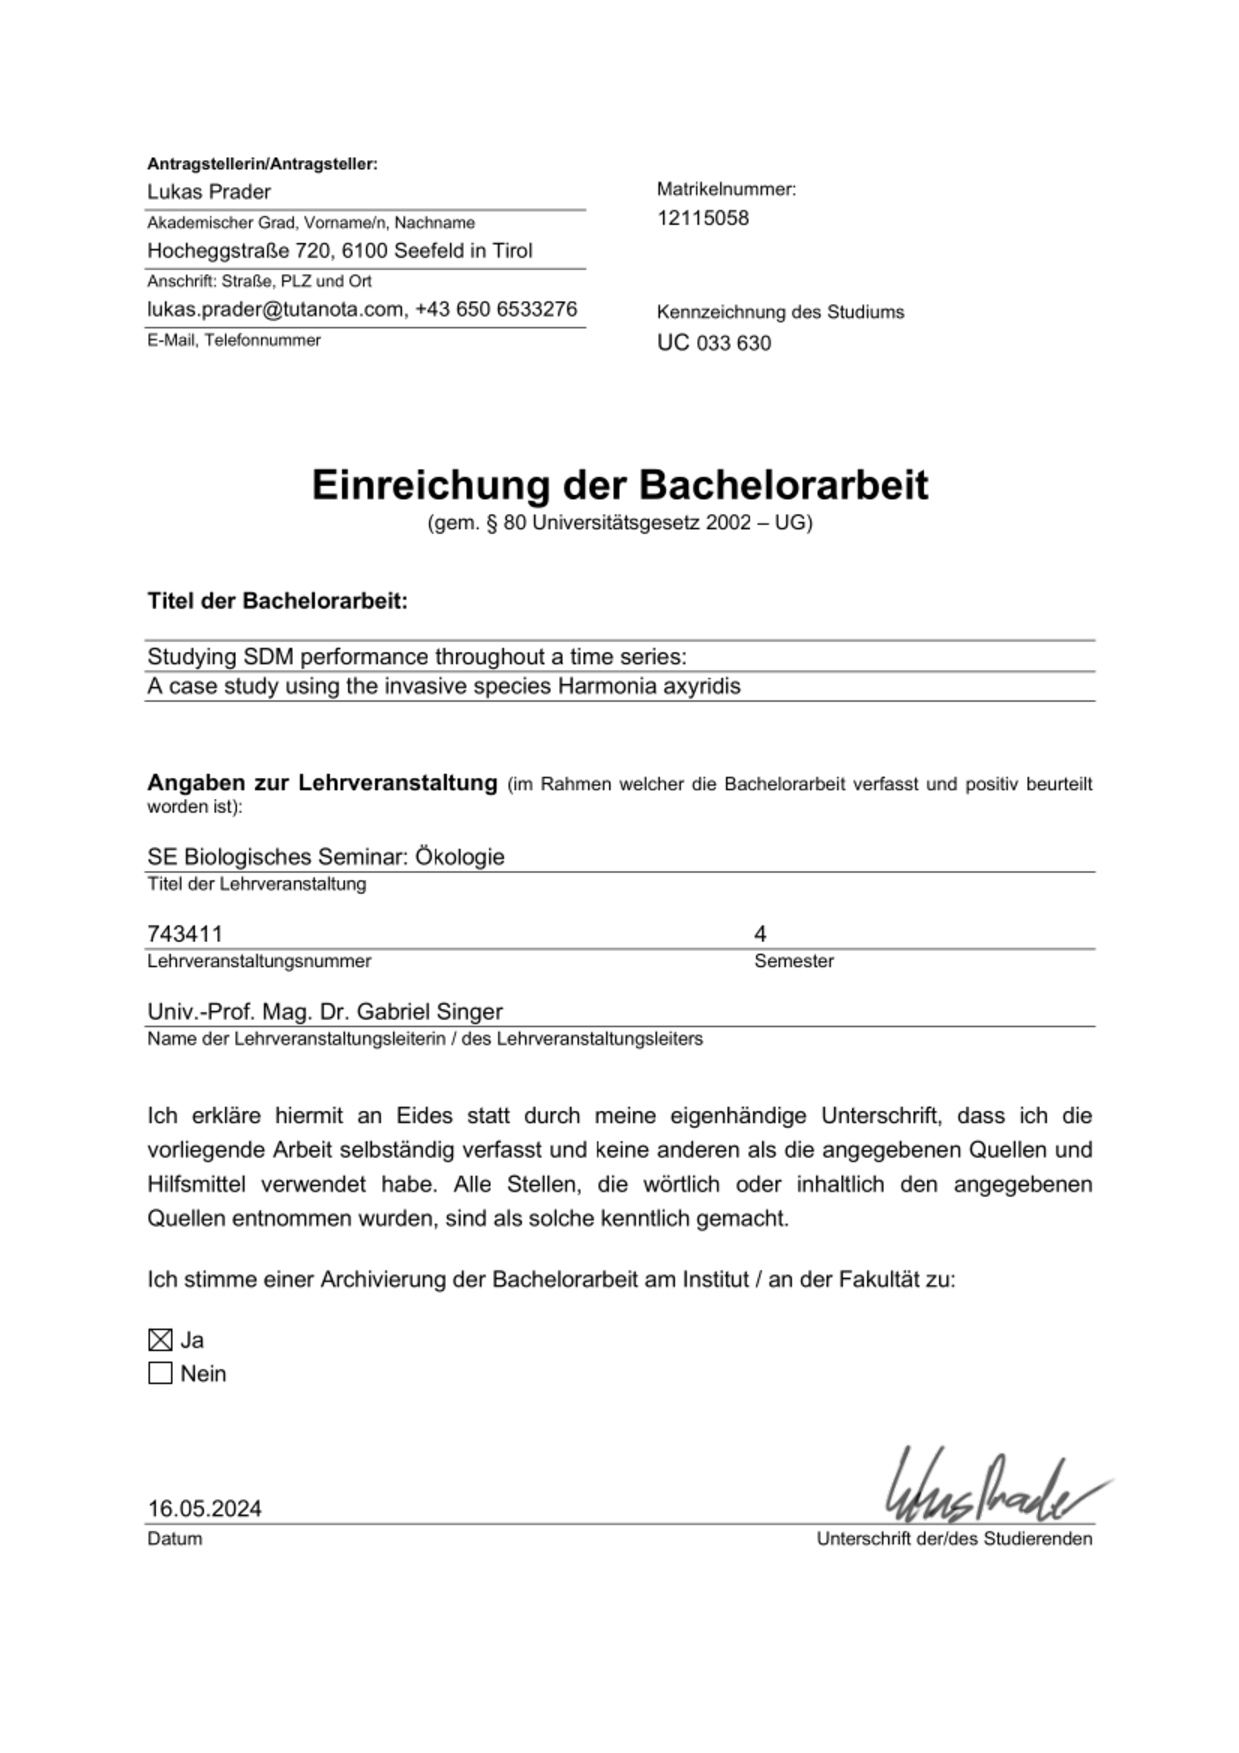
\includepdf[pages=-]{einreichung_bachelorarbeit.pdf}
%Einverstaendnis mit Veroeffentlichung der Bachelorarbeit
\thispagestyle{empty}
I, Lukas Prader, agree that my bachelor's thesis (``Studying SDM performance throughout a time series: A case study using the invasive species \textit{Harmonia axyridis}''), mainly supervised by Dr. Lauren Talluto, will be digitally archived in a repository of Leopold Franzens University Innsbruck and made available for further academic use. \\

Innsbruck, \findate					\hfill Signature  \includegraphics[height = 10mm]{"signature.png"}

%title page
\newpage
\thispagestyle{empty}
\begin{center}
    \Large{University of Innsbruck \\ Faculty of Biology} \\
    \vspace{3mm}
    \large{Department of Ecology}
    \vspace{10mm}

    \includegraphics[width = 0.6 \linewidth]{universitaet-innsbruck-logo-cmyk-farbe.jpg}

    \vspace{10mm}
    \Large{Bachelor Thesis} \\
    \large{submitted for the degree of} \\
    \Large{Bachelor of Science} \\
    \vspace{10mm}
    \LARGE{\textbf{Studying SDM performance throughout a time series: A case study using the invasive species \textit{Harmonia axyridis}}} \\
    \vspace{10mm}

    \large{by \\ Lukas Prader \\ Matriculation Nr.: 12115058 \\ SE Biological Seminar: Ecology}
\end{center}

\vspace{30mm}
\begin{tabular}{ll}
    \large{Submission Date:} & \large{\findate}                       \\
    \large{Supervisors:}     & \large{Lauren Talluto, Gabriel Singer} \\
\end{tabular}

\newpage
\thispagestyle{empty}
\begin{abstract}
    \noindent In invasive ecology, a lot of research is aimed at predicting the potential impact that a species could have outside its native range.
    Species Distribution Models (SDMs) have been applied in this context already, but with still ongoing discussion of their actual viability given the dynamic aspect of niches in the process of invasion.
    To further insight into the applicability of SDMs for predicting invasive species, a SDM ensemble time series modelling the European niche of \textit{Harmonia axyridis} over the time period 2002-2020 was created.
    In addition, niche dynamic analyses were conducted, computing the niche stability and expansion over time among other parameters.
    It was shown that SDMs trained on data only from the invaded range achieve consistently high model sensitivity, and this in the context of an almost completely stable niche over the whole time period.
    Models with data only from the invaded range, as well as models using native data only are consistent with previous work predicting the range of \textit{H. axyridis}. \\

    \noindent Keywords: Species Distribution Model, invasive species, ensemble model, time series, niche dynamic analysis, ecospat
\end{abstract}

\newpage
\tableofcontents
\thispagestyle{empty}
\newpage
\pagenumbering{arabic}

\section{Introduction} \label{sec:introduction}
% Invasion Theory
Invasive species are of special interest in ecological research due to their impact on native ecosystems.
Main goals in this area are to find out which species have potential to become invasive, what habitat will be susceptible to invasion by those species, how fast the species will invade the new area and what impact its invasion will have on the native ecosystem \autocite{shigesada1997invasions}.
To this end, many theories have been created to describe invasion processes.
The invasion of a species can  generally be described with four stages \autocite{blackburn2011invasionstages}:
\begin{enumerate}
    \item Transport: Leaving the native range, arriving at a new location
    \item Introduction: Existing in specific locations (captivity / cultivation)
    \item Establishment: Existing outside of areas of introduction in the wild
    \item Spread: Sustaining establishment and dispersing to new environments
\end{enumerate}
Depending on the current stage there can be significant differences in behaviour and impact of a species.
The impacts of invasive alien species can be numerous, ranging from food web changes to reductions in habitat and species richness, hydrology and nutrient cycle changes, enhanced invasion of other species and extinctions \autocite{simberloff2013invasiveimpacts}.
For example intraguild predation, the predation of species using similar resources, can create completely new stable states of an ecological system \autocite{polis1989theoryIGP}.
Fully understanding the dynamics at play during the invasion process would open more possibilities to actively influence the invasion of threatening species.
For this, creating models which are able to predict the invasion is one current focus of research.
Since invasion theory already uses niche theory, it is quite appropriate to think about applying niche models to the problem.

% SDM Theory
Species Distribution Models (SDMs), are being applied to predict the further development of species occurrences in many contexts, also for invasions.
These types of models have been shown to generate substantial insight into the ecological requirements of species and, as niche models, can be used to predict the potential habitat of a species \autocite{araujo2006sdmchallenges}.
There has been considerable debate on the capabilities and limitations of SDMs, especially when used for prediction outside the data domain.
In general, SDMs are made with the (ideal) assumption that the species is in environmental equilibrium \autocite{elith2009sdmtheory}, implying that its ecological niche is not currently changing.
If these models are now used to predict new, unsampled regions, there actually is no measure to assess their accuracy, since no data is presently available for that area \autocite{araujo2006sdmchallenges}.
This means that when trying to predict areas which are potentially outside the calibration range, sufficient validation data is lacking, implying strong uncertainty about the predictive performance of a given model \autocite{araujo2006sdmchallenges}.
This issue of model transferability is an ongoing area of research in the SDM community.
There is also no guarantee that the biotic interactions sampled in the study area will reflect the final interactions in the new area \autocite{elith2009sdmtheory}.
In many cases it has been shown that invasive species suffered less from parasites or other natural enemies in the invaded range, for example making it easier for them to become pests with negative impact (Enemy Release Hypothesis, \autocite{williamson1996bioinvasions}).
All of these issues apply especially to the prediction of invasive species, since there might be limited data in the invaded range, the species is often not currently at equilibrium and interactions with native species are completely new \autocite{mainali2015sdmprojecting}.
Despite all these challenges, SDMs have been used numerous times to provide insight into the invasive potential and the invasion dynamics of alien species \autocite{zimmermann2010sdmtrends}.
One way of gaining more insight into the invasion process is to create models with data from different time periods during the invasion \autocite{briscoe2019palmerisdm}.
For example, data from a time period early in the invasion process can be used to build models which then are evaluated against data from a later time period \autocite{barbet2018nigrithoraxsdm}.
With this, SDMs can be used to detect niche shifts, which in turn improves the understanding of the underlying niche dynamics and their impact, which helps to put model performance into perspective, for example when using its results for risk assessment of potential invasions \autocite{pearman2008nicheSDM}.

% Modelling Method
SDM performance is not only influenced by the underlying data, but also the type of model chosen for the analysis.
Models range from regression methods to machine learning and each feature various strengths and weaknesses, possibly leading to vastly different results for the same dataset \autocite{valavi2022SDMperformance}.
Due to those differences, a possible approach is to create an ensemble of multiple models \autocite{araujo2007ensemble}.
The way of combining model predictions can vary, but the goal is to improve total performance by combining the results of all computed models.

% Harmonia axyridis
In order to conduct an iterative modelling approach, a species with sufficient data over the time span of invasion is necessary.
\gls{harm}, also known as the Harlequin ladybird or multicoloured Asian lady beetle, is of the family of the Coccinellidae and has its native origin in Asia \autocite{roy2016harmonia}.
At the time of download, the GBIF dataset for \gls{harm} consisted of 468.462 data points globally, resulting in very sufficient amounts of data (see \ref{ssec:temp_data_change}).
At first widely introduced as a control species against pest aphids, \gls{harm} has turned out to be a highly invasive species reaching an almost global distribution \autocite{brown2008harmonia}.
In America, the species was introduced as early as 1916 (California) and in 1988, first populations outside intended release were found \autocite{chapin1991harmoniaNA}.
Usage of \gls{harm} for biological control in Europe dates back as far as 1990 (France) \autocite{coutanceau2006harmoniaFR}.
First invasive occurrences were confirmed in multiple countries during the early 2000s, including Germany (2000), Belgium (2001), the Netherlands (2002) and the United Kingdom (2003) \autocite{roy2016harmonia}.
The first confirmation in Austria, where it was never used for biological control, was in 2006 \autocite{rabitsch2006harmoniaAT}.
It has been shown that all established invasive populations outside of North America have their origin in the first established population in eastern North America, with the European populations being significantly influenced by the used biocontrol strain \autocite{lombaert2010harmoniabridgehead}.

The impact of \gls{harm} on invaded areas is diverse.
In some contexts, the ladybird has been shown to have a negative impact on the diversity and abundance of native ladybird species \autocite{roy2016harmonia}.
Many studies show intraguild predation and direct interspecific competition in favour of \gls{harm} \autocite{pell2008harmoniaIGP}.
This results in a large potential for \gls{harm} to be a significant threat for guild diversity and community structure in its introduced ranges.
It has also been shown that the species feeds on a variety of damaged fruit crops, for example grapes, apples, stone fruit and berry crops, making it a pest in these scenarios \autocite{koch2004harmoniafoodcrop}.
The aggregating behaviour of \gls{harm}, mostly as a strategy for overwintering, is also a cause of disturbance, since private homes and facilities are invaded by large amounts of beetles at a given time \autocite{nalepa2005harmoniahomes}.
In general, \gls{harm} can be concluded to be a species with high impact as an invader, and thus of interest for active research questions.

%existing SDMs for H. axyridis
There have been several publications which modelled and predicted the distribution of \gls{harm}, constrained to certain geographical ranges (i.e. Spain \autocite{ameixa2019harmSDMSpain}, Chile \autocite{alaniz2018harmSDMChile}) or even on global scales \autocite{bidinger2012harmSDMglobalMaxent, poutsma2008harmSDMglobalClimex}.
There has not yet been any model iteration in form of a time series, which is what this thesis aims to add as new insight.
Another goal of this thesis is to look into the limitations of models built early in the invasion process of a species.
By iterating over the years of the invasion, model performance can be evaluated with consideration to the current state of invasion.
In the end, a better understanding of the invasion process of \gls{harm} in Europe and the performance of models trying to capture it should be the result.



\newpage
\section{Materials and Methods} \label{sec:materialsandmethods}

\subsection{Datasets} \label{ssec:datasets}
For occurrence data, all global occurrences of \gls{harm} were downloaded from the GBIF database \autocite{GBIFaxyridisdataset}.
All traditional 19 bioclim variables, which mostly concern mean temperature, precipitation and different kinds of their variation (see Supplementary Table \ref{tab:bioclim} for full breakdown), were obtained from the CHELSA V2.1 climatologies dataset \autocite{karger2017CHELSApaper, CHELSAbioclimdataset}.
The 1981-2010 time frame was used for all years from 2002 to 2010, the MPI-ESM 1.2 ssp370 scenario 2011-2040 for all years from 2011 to 2022.
As additional information, land cover data was used from the Copernicus Land cover Classification dataset \autocite{COPlandcoverdataset}  with yearly resolution for 2002 up to 2020.
For all used occurrence points after 2020, the land cover data of 2020 was used, since at the time of this thesis data for 2021 and 2022 was not yet available.

\subsection{Data preparation} \label{ssec:datapreparation}
All bioclim and land cover layers were resampled to a matching resolution of 30 arc seconds and cropped to two spatial extents, Europe and the presumed native range \autocite{orlova2015harmonia}.

The presence-only points from GBIF were checked for missing values for latitude, longitude, year or coordinate uncertainty and then subsetted to the aforementioned spatial extents.
No occurrences after 2022 were used, also no points with a coordinate uncertainty larger than 1 km, which is approximately the latitudinal resolution of the raster data.
In Europe, the initial cut off year for presences was 1991, since this is the year of invasion according to the EASIN website \autocite{EASINintroharm}.
Afterwards, using the library \texttt{CoordinateCleaner} \autocite{zizka2019coordinatecleaner}, all remaining data points were again checked for common errors or biases in the respective subset.
The tests used check for occurrences too close to country capitals (``capitals''), country centroids (``centroids''), duplicates or points with equal absolute coordinates in both dimensions (``duplicates'', ``equal''), as well as points close to biological institutions (``institutions''), geographical outliers (``outliers''), points located in oceans (``seas'') and points with equal longitude and latitude or close/equal to the point (0,0) (``zeros'').
In addition, all occurrences were checked for their land cover class values in their respective year, removing points in the water or with no data.
In the end, remaining data points prior to 2002 were deemed insignificant and removed from the dataset.
This resulted in a total of 124.746 presence points over all years and areas.
To prepare the data for modelling, pseudo-absences were generated for each year, randomly sampling the area, discarding and re-sampling points in the water or with no data.

To correct for sampling bias in the data, the European and native extents were split into sub-extents in order to add additional absences to more densely sampled regions, attempting to re-create the sampling bias for the pseudo-absences \autocite{phillips2009samplebias}.
For this, an algorithm was written which splits a given extent in half and continues to do so with the created sub-extents until the amount of points in the extents is at most some chosen number.
For the first part of absence generation completely random absences are drawn from the original extent in order to ensure at least some coverage of the whole study area.
In the second step, additional absences are generated for each sub-extent separately and in relation to the amount of presences inside the respective sub-extent.
This results in more absences in regions with more presences as well (Fig. \ref{fig:ext_subdiv} A).
The subdivision of the dataset was carried out using all presences in Europe over all years and setting the threshold to be $\leq$ 30\%, leading to sub-extents converging around the United Kingdom and the Netherlands, which seem to have been sampled very intensely (Fig. \ref{fig:ext_subdiv} B).
This bias probably originates from the nature of the invasion, with \gls{harm} seemingly having multiple fronts and degrees of severity during establishment.
For the first and second step of absence generation, absences equal to and twice the amount of presences were generated respectively, resulting in three absences per presence in total.

\begin{figure}[!h]
    \centering
    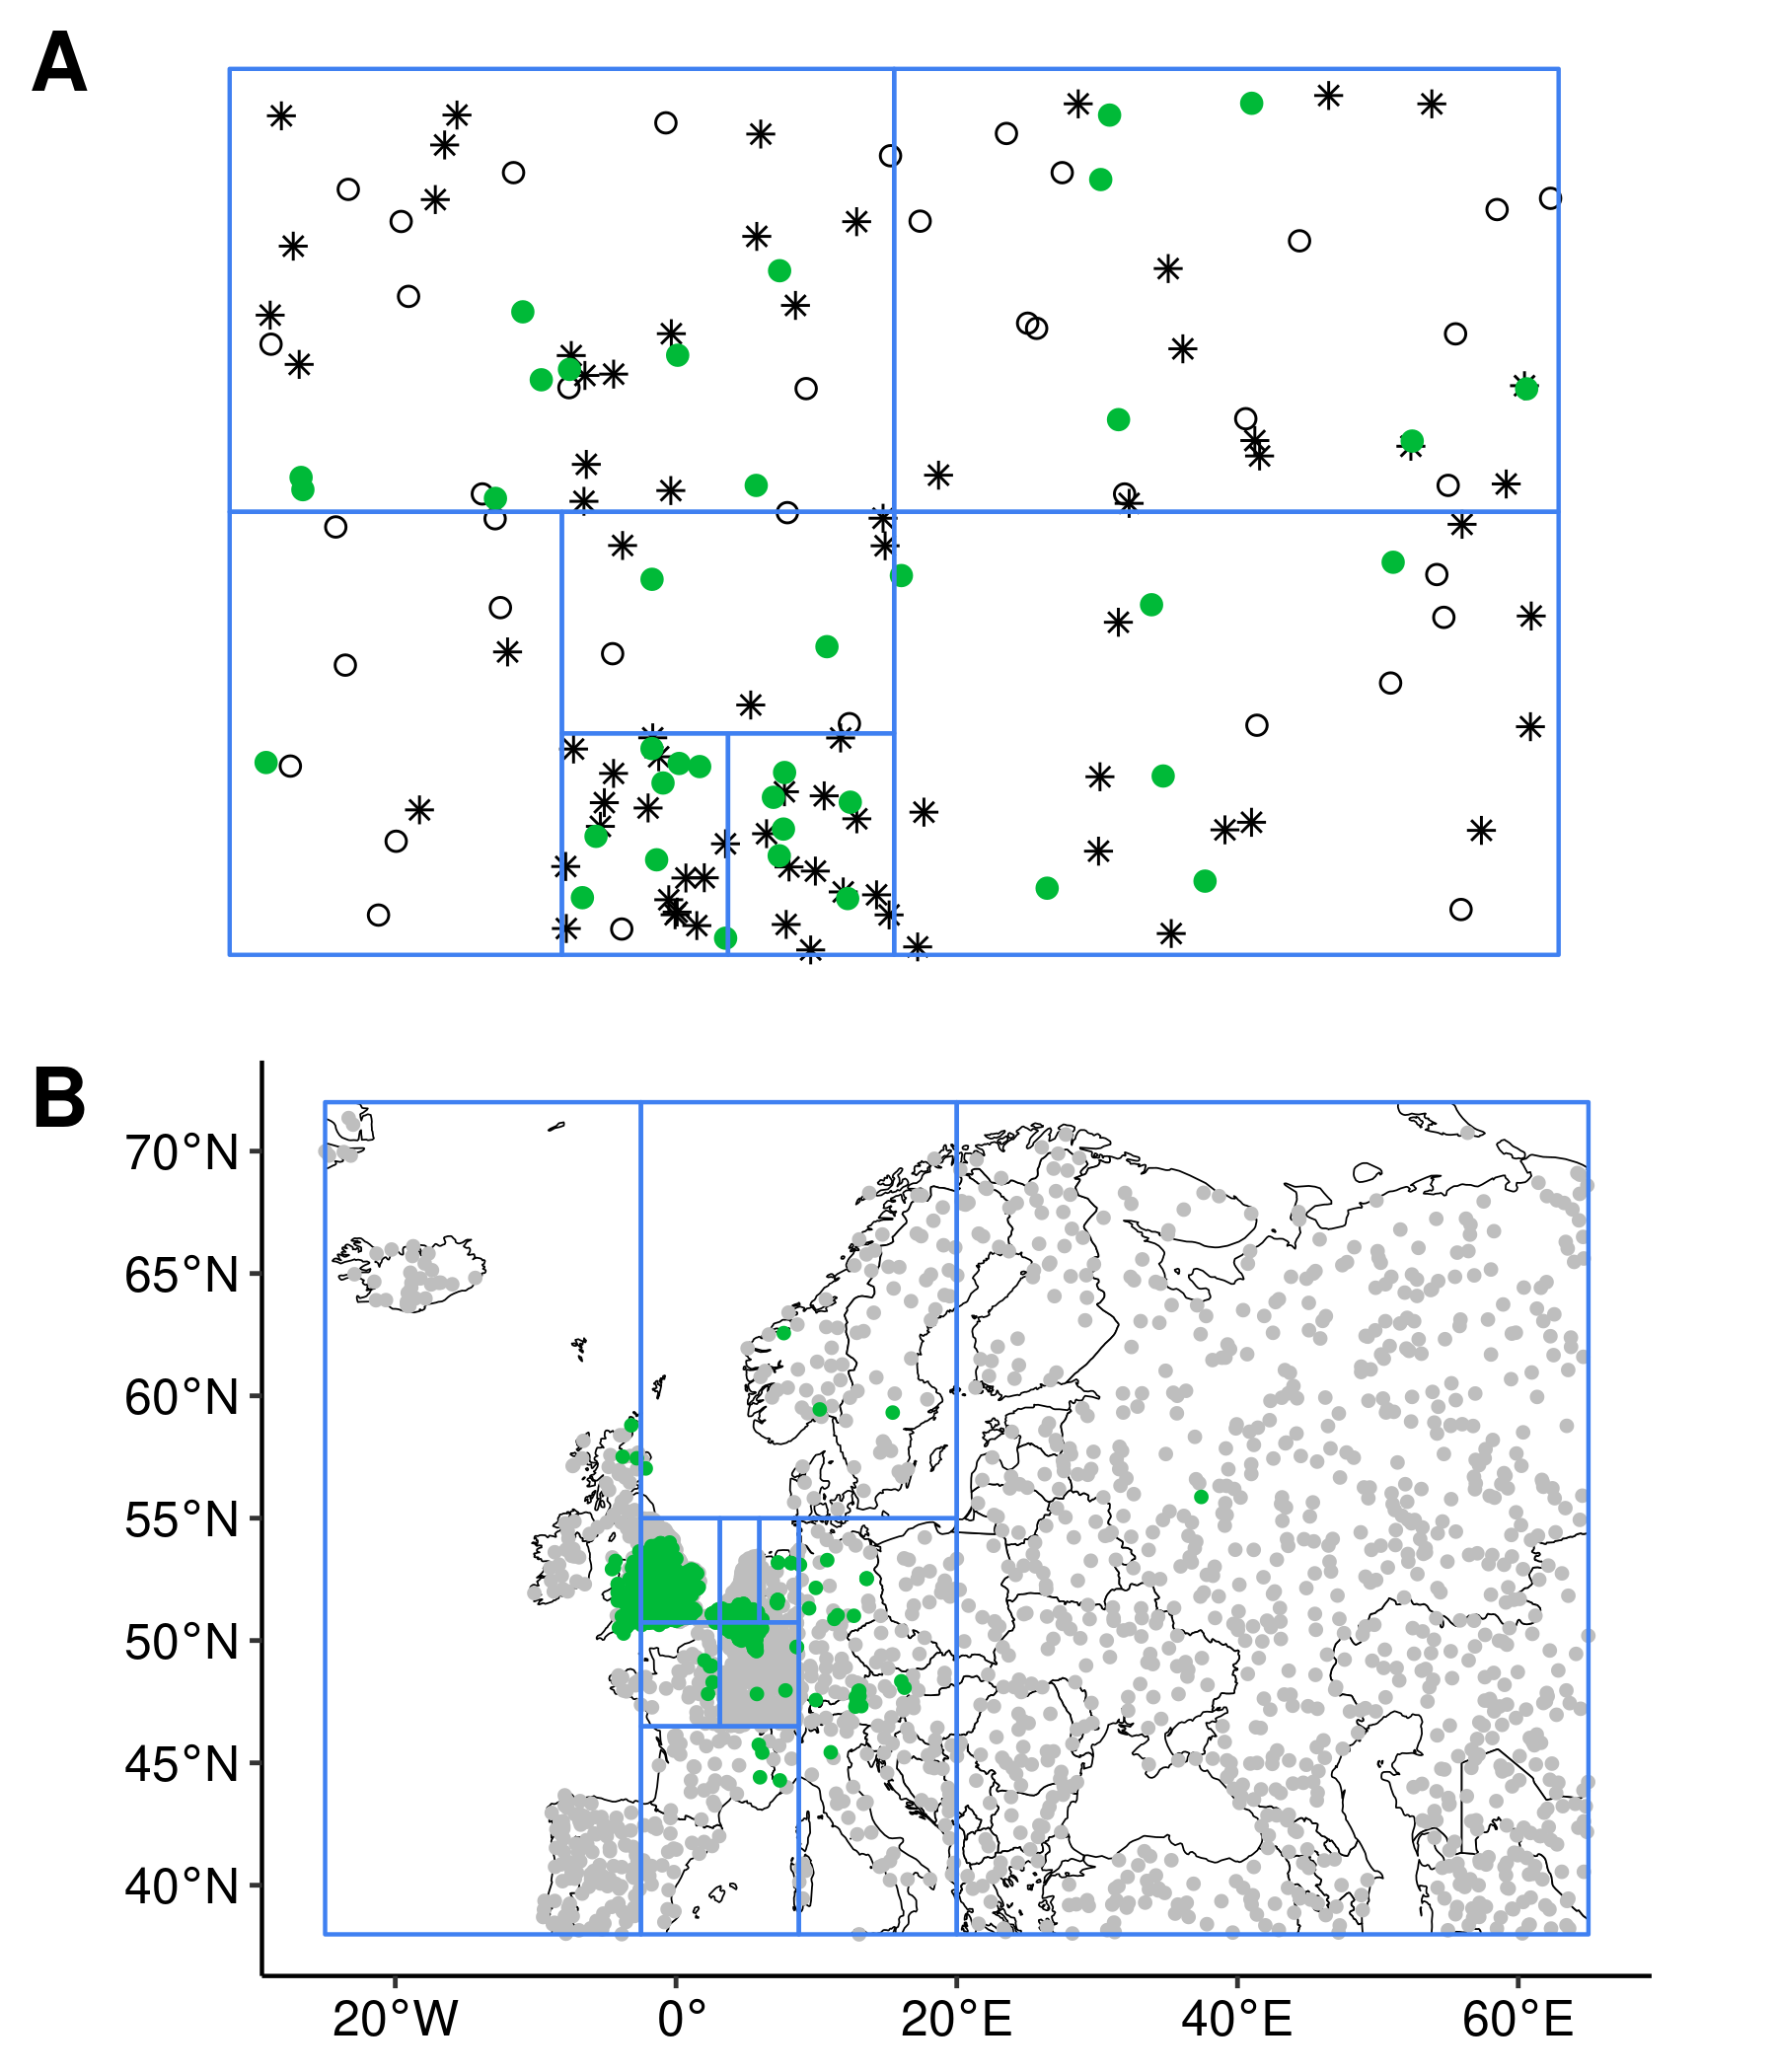
\includegraphics[width = 0.8\linewidth]{"../../R/figures/ext-subdiv.png"}
    \caption{\label{fig:ext_subdiv} Visualization of the subdivision algorithm and absence generation. Subfigure A shows an example of 30 generated presences (green), subdivided with a threshold of $\leq$ 10 points per sub-extent. The generated absences are shown in black, with circles indicating the first 30 completely random absences, and asterisks indicating absences generated relative to the amount of presences in a sub-extent. Subfigure B shows the calculated sub-extents for the total presences of the dataset, with presences (green) and absences (grey) for 2008 plotted as an example.}
\end{figure}

\subsection{Model building} \label{ssec:modelbuilding}

In order to evaluate the impact of the invasion process on SDM predictive performance for \gls{harm}, multiple models were compared: General Linear (GLM) \autocite{guisan2002glm-gam}, General Additive (GAM) \autocite{guisan2002glm-gam}, Boosted Regression Trees (BRT) \autocite{elith2008brt} and Maximum Entropy (MAXENT) \autocite{phillips2017maxnet}.
A model for a specific year always included all points from past years as well.
The iterative models that were built only use data points from Europe, though there was one model created only with native occurrences and predicted for each year in Europe.
This is to compare performance between models with and without potential influences of a niche shift through the process of invasion.
The four built models were then used to create a weighted ensemble (see \ref{ssec:analysis}) using the sensitivity of the models.

Variance inflation factors were used to select the variables used for model building.
For this, a GAM was computed only using Europe data from 2002, using all bioclim and land cover variables.
For land cover variables, a PCA was computed on the relative area of all land cover classes in an 18 km radius around 5000 random data points in Europe, subsequently projecting the occurrence data onto the resulting axes.
The 18 km radius was chosen, since it is the average flight distance determined for \gls{harm} \autocite{jeffries2013flightharmonia}.
PCA axes were included in the model until a cut-off of 80\% of explained variance was reached.
Variance inflation factors were computed for this GAM and the variable with the highest VIF was dropped until none of the remaining variables had a VIF greater than 10 (rule of ten, see \cite{obrien2007cautionVIFs}).

\subsection{Analysis} \label{ssec:analysis}
All SDM models of each year were evaluated for their accuracy on predicting the occurrences of the following year using sensitivity.
The sensitivity values were used to create a sensitivity-weighted ensemble (weighted sum) of all model predictions, which was again evaluated for its accuracy.
The thresholds used to compute sensitivity were computed using the library \texttt{PresenceAbsence} \autocite{freeman2008presenceabsence}, choosing the option which maximizes $(Sensitivity + Specificity) / 2$.
This will also maximize the True Skill Statistic $Sensitivity + Specificity - 1$, which is a commonly used performance metric for SDMs \autocite{leroy2018TSSissues}.
This thresholding was chosen since just maximizing sensitivity can be achieved trivially by setting the threshold as low as possible, creating a model which predicts everything as suitable (used thresholds in Supplementary Table \ref{tab:mod_ths}).


A series of niche analyses was conducted using the library \texttt{ecospat} \autocite{dicola2017ecospat}.
For each year, the occupied niche was computed by running a PCA analysis on the bioclim variables.
The niche was then visualized by plotting a dynamic occurrence density grid for the first two PCA axes \autocite{broennimann2012niche}.
Niche overlap between the total EU data and the total native niche was also visualized.
In order to compare the similarities or differences between the native and invaded niche, two tests were performed, namely a niche equivalency test and a niche similarity test \autocite{broennimann2012niche}.
With the niche equivalency test, one determines if the niche overlap stays constant while randomly sampling from pooled observations of each niche and calculating the overlap \autocite{broennimann2012niche}.
When conducting the niche similarity test, one tests if the observed niche overlap is different from that of niches sampled randomly from their respective available environments (backgrounds) \autocite{broennimann2012niche}.
These tests have very different implications, with equivalency asking if two niches are ``identical'' in the sense of constant overlap, and similarity concerning the overlap compared to the possible overlaps in the given environment.
One could imagine a case, for example a small island, where the niche equivalency test is significant, but the niche similarity test fails since the available environments are so similar that the two niches naturally overlap.
For this reason it makes sense to perform both tests in a general case.


The niche similarity test differs from the equivalency test
because the former examines whether the overlap between
observed niches in two ranges is different from the overlap
between the observed niche in one range and niches selected at
random from the other range. In other words, the niche similarity test addresses whether the environmental niche occupied
in one range is more similar to the one occupied in the other
range than would be expected by chance.

The overlap between each year for Europe and the respective following year was computed using Schoener's D metric, which compares the occupancy of grid cells of the compared niches and ranges from 0 to 1.
Additional niche dynamic indices, ``stability'', ``expansion'' and ``unfilling'' \autocite{guisan2014nichedyn} were also computed.
These correspond to the relative amount of shared, only native and only invaded area of niche space in the context of an invaded niche being compared to its native counterpart.



Finally, the development of sensitivity over time was tested for correlation with the amount of training data and the niche stability for a given year, using the Pearson correlation test.

\newpage
\section{Results} \label{sec:results}

\subsection{Temporal change of data availability} \label{ssec:temp_data_change}
After cleaning the data, the number of presences proved to consistently be higher in the European range compared to the native area, with the number of presences increasing exponentially over the studied time period for both areas respectively (Fig. \ref{fig:pres_per_year_log}).

\begin{figure}[!h]
    \centering
    \includegraphics[width = 0.9\linewidth]{"../../R/figures/pres-per-year-log.png"}
    \caption{\label{fig:pres_per_year_log} Number of presence points for \gls{harm} by year and area, using the cleaned dataset (Supplementary Fig. \ref{fig:raw_vs_cleaned_glob}).}
\end{figure}

With at least 100 presences for any year, the European dataset is definitely sufficient to create SDMs for each year separately, more so if data from previous years is also used.
The exponential increase in observations (in later years) is most likely due to an increase in sampling effort, since native observations grow at the same rate.
The lack of presence points in early years in the native range was the reason why it was decided to only create one SDM with the native data of all years combined, since it is more likely to provide a complete evaluation of the native niche.

\subsection{Niche dynamic analysis} \label{ssec:niche_dyn_analysis}

\begin{figure}
    \centering
    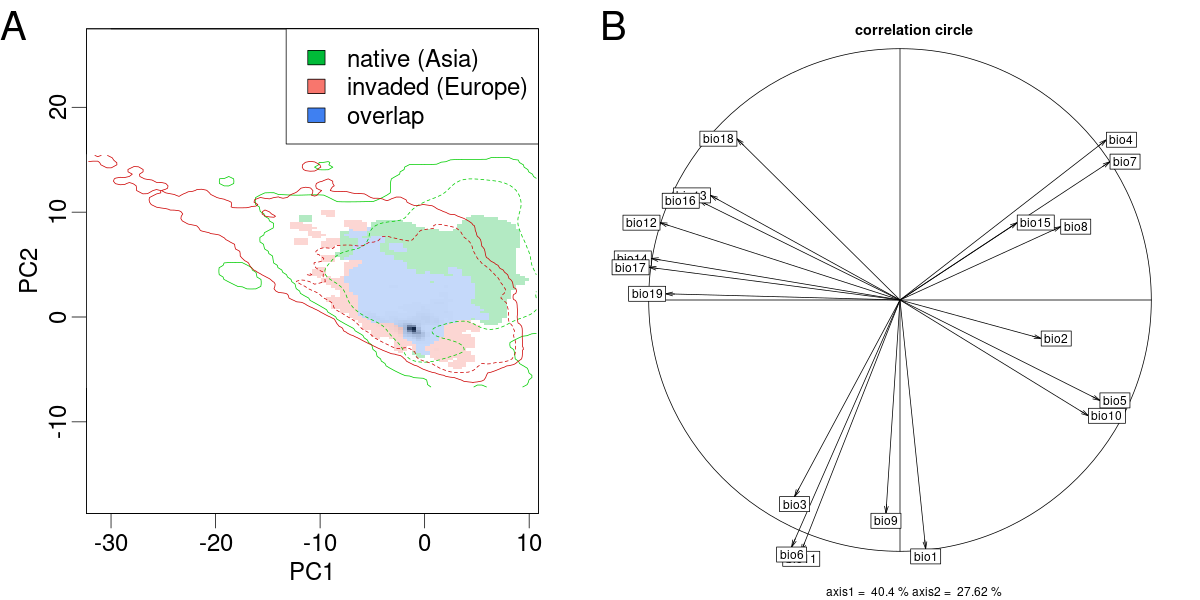
\includegraphics[width = 1\linewidth]{"../../R/figures/as-eu-tot-niche-w-pca.png"}
    \caption{\label{fig:as_eu_niche_w_pca} (A) Native (green) and invaded (red) niche of \gls{harm}, shown along the first two axes of a PCA (B) using all bioclim variables. The blue area indicates overlap between the occupied niches. Dashed and solid lines indicate 50\% and 100\% of the potentially available environment in each area (environmental density quantiles of background). Grey shading shows the density distribution of the invaded niche. For detail on the bioclim variables, see (Supplementary Table \ref{tab:bioclim}).}
\end{figure}

When comparing the total native and invaded niches (i.e., all years included), the niches are clearly different (Fig. \ref{fig:as_eu_niche_w_pca}).
A niche similarity test produced a p value of $p = 0.32$, leading to an accepted null hypothesis meaning the two niches are not more similar than random, given the environment (Supplementary Fig. \ref{fig:as_eu_eq_sim}).
Conducting a niche equivalency test, the result was $p = 0.01$ implying highly significant differences between the two niches (Supplementary Fig. \ref{fig:as_eu_eq_sim}).

Looking at the niche only in the invaded range, one can visualize the shift and expansion throughout the years (Fig. \ref{fig:eu_niche_ys}).

\begin{figure}[!h]
    \centering
    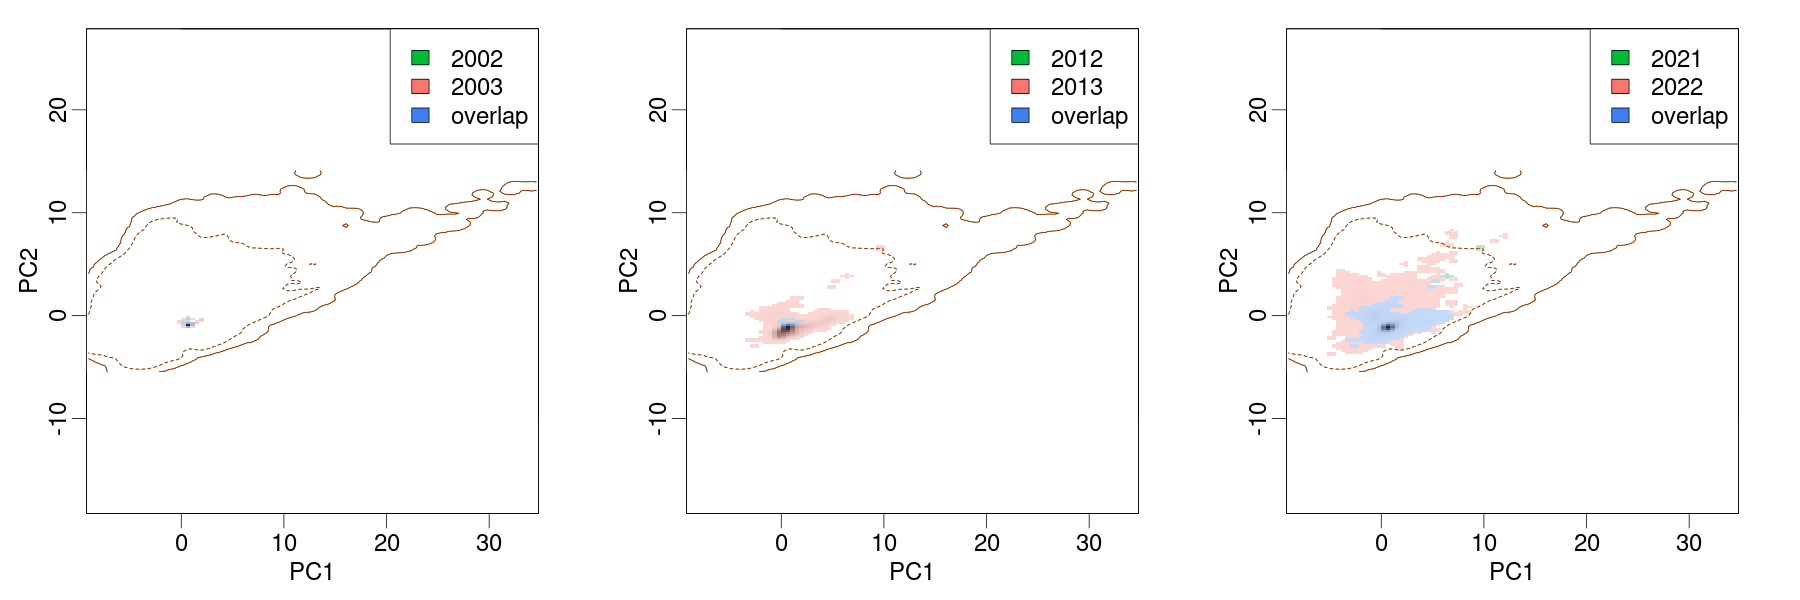
\includegraphics[width = \linewidth]{"../../R/figures/eu-niche-ys.png"}
    \caption{\label{fig:eu_niche_ys} The progression of the invaded niche of \gls{harm}, shown along the first two axes of a PCA using all bioclim variables (Supplementary Fig. \ref{fig:eu_years_pca}). Niches of the years (from left to right) 2002, 2012 and 2021 compared to the niche of their following years respectively. Green shows the first year, red shows the year after and blue indicates overlap. Dashed and solid lines (brown due to overlap) indicate 50\% and 100\% of the potentially available environment (environmental density quantiles of background). Grey shading shows the density distribution of the second year.}

\end{figure}

In addition to a visualization, it makes sense to compute the niche dynamic indices \autocite{guisan2014nichedyn}, as well as the niche overlap (Schoener's D) for each year in order to characterize the niche shift further (Fig. \ref{fig:eu_niche_dyn}).

\begin{figure}[!h]
    \centering
    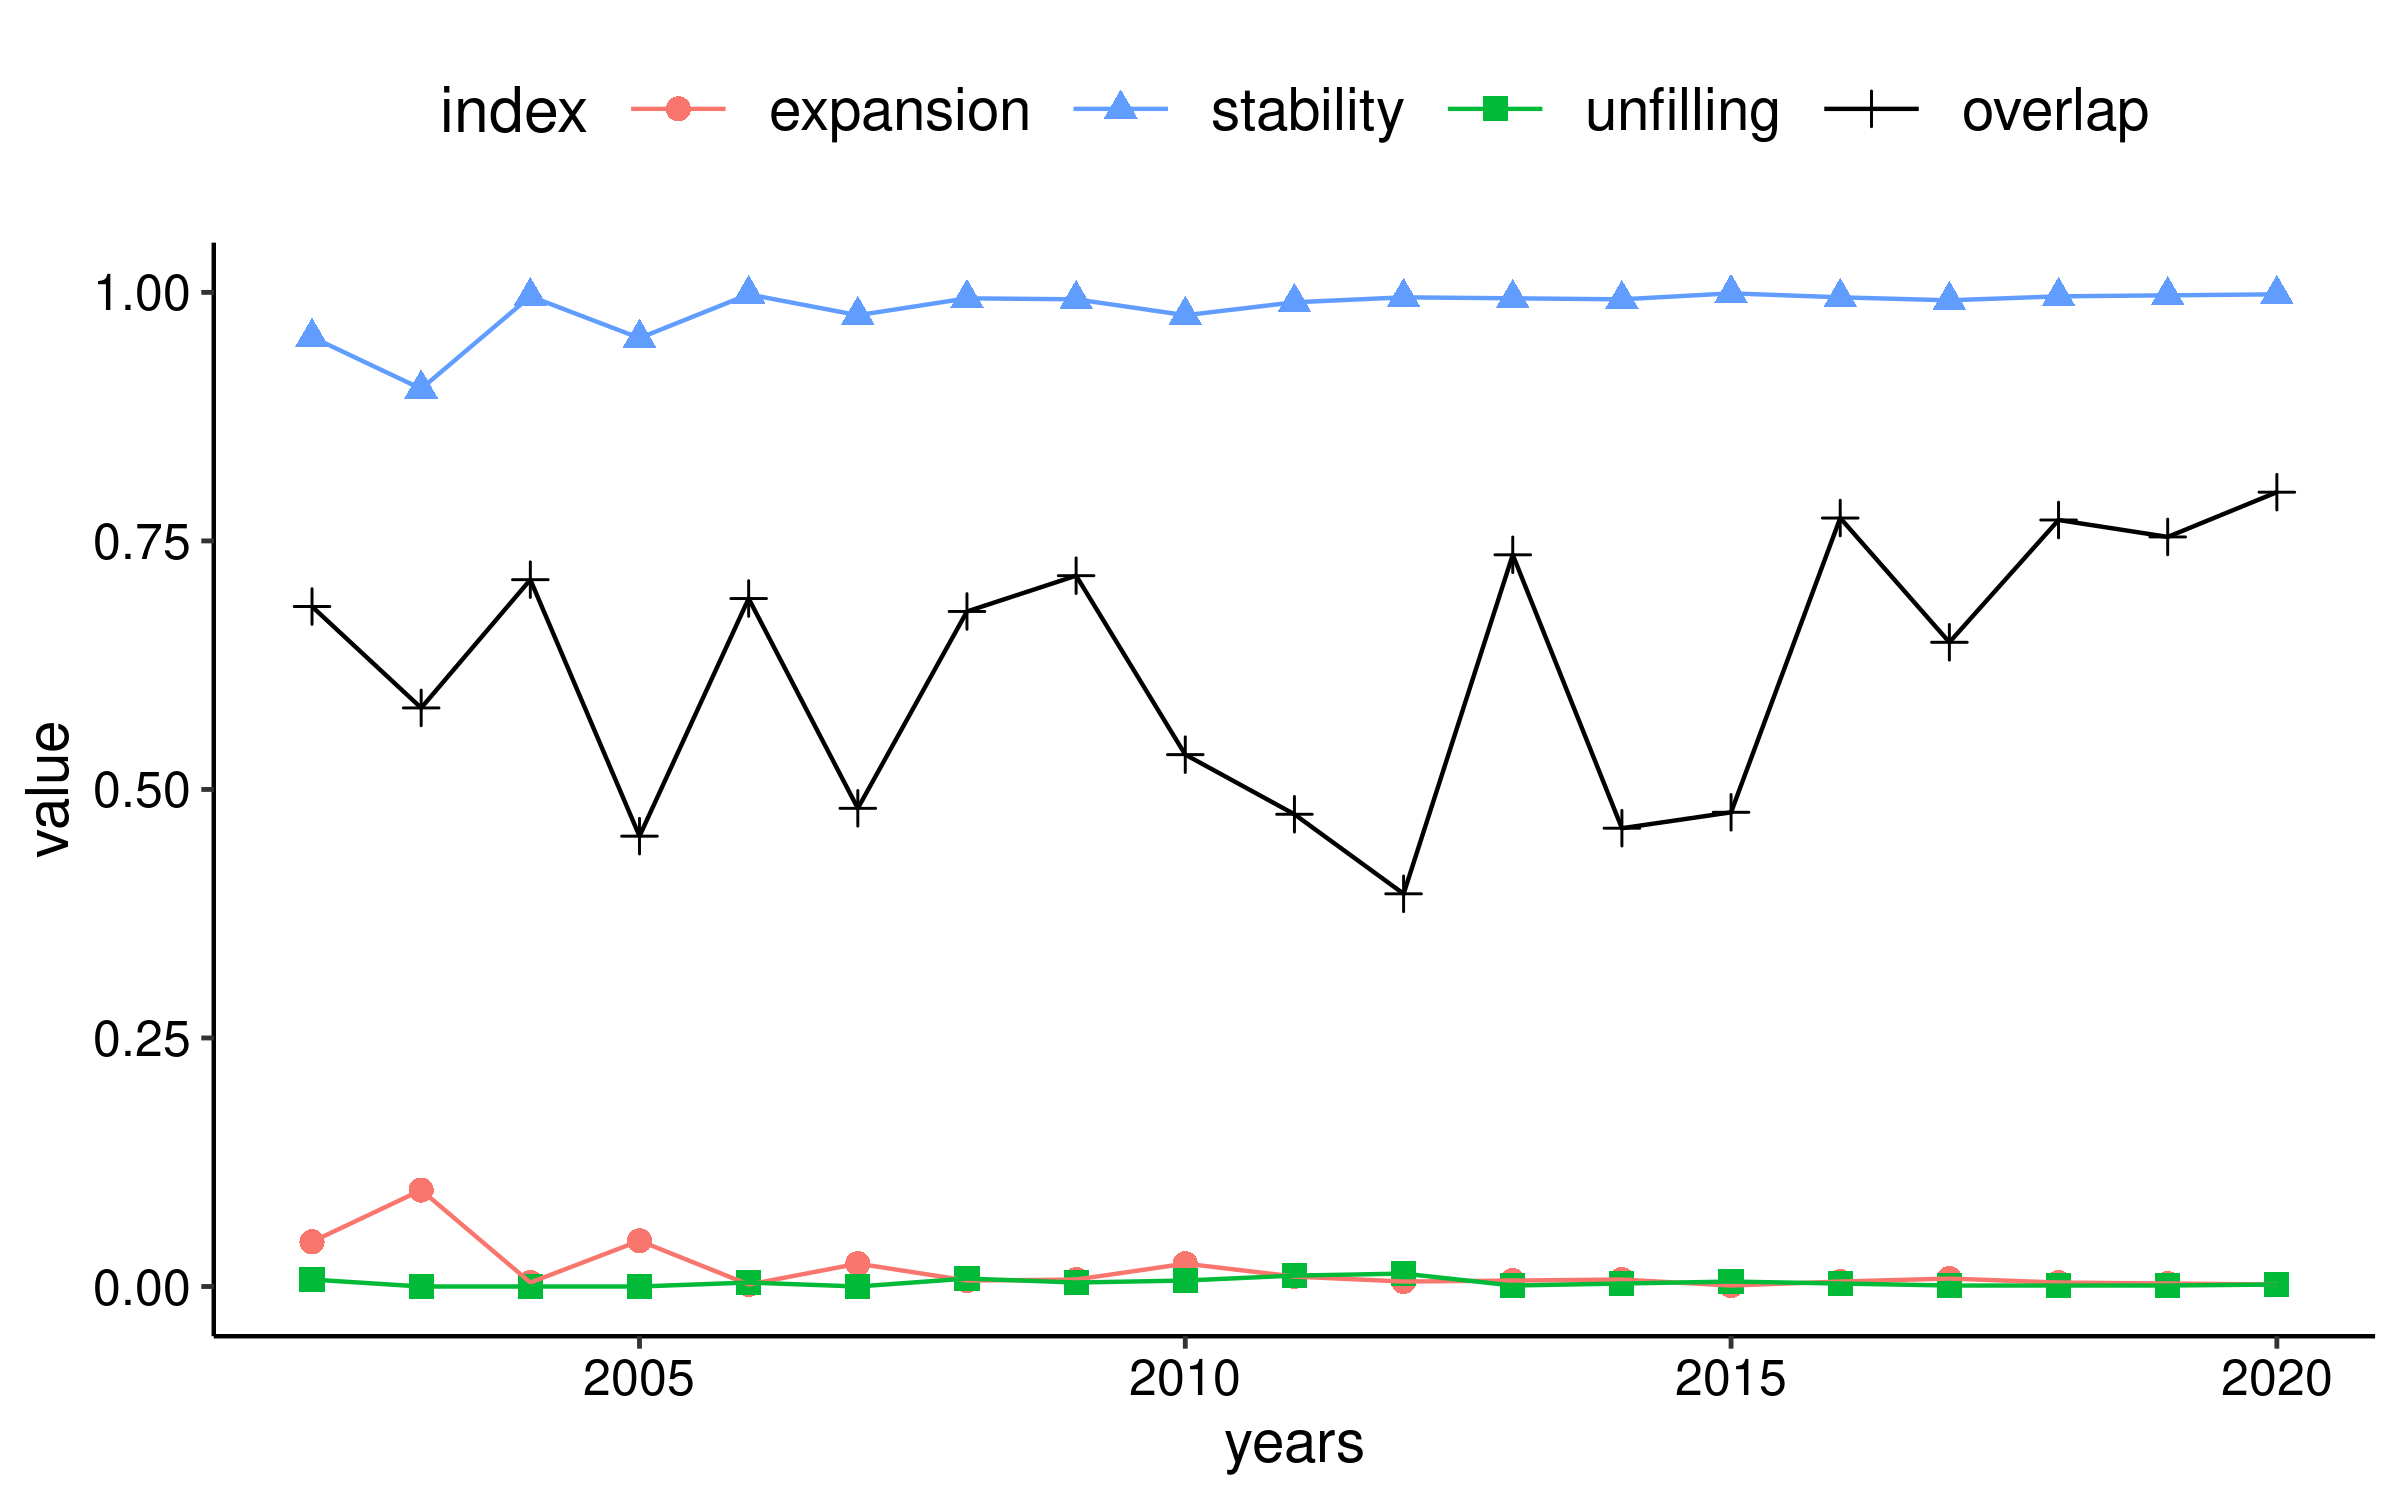
\includegraphics[width = 0.9\linewidth]{"../../R/figures/eu-niche-dyn.png"}
    \caption{\label{fig:eu_niche_dyn} Niche dynamic indices and overlap (Schoener's D) computed from comparing each year of the invaded niche of \gls{harm} to the following year.}
\end{figure}

The results show that in the first five years of the time series, the invaded niche is still expanding, while afterwards it becomes almost completely stable.
Once stability is reached, \gls{harm} seems to just fill out the rest of the acquired niche, as shown by an increase in niche overlap.

\subsection{SDMs, ensemble and time series}
Variable selection using VIFs resulted in 13 variables, which were used for modelling (Table \ref{tab:var_vifs}).

\begin{table}[!h]
    \centering
    \caption{\label{tab:var_vifs} Final 13 variables resulting from variable selection with VIFs, PCA contribution table for all land cover variables in (Supplementary Table \ref{tab:lc_contrib}), bioclim variable explanation in (Supplementary Table \ref{tab:bioclim})}
    \centerline{
        \begin{tabular}{l| r*{13}{ c}}
            \csvreader[no head, column count = 14, late after line = \\]{tab-var-vifs.csv}{}{\csvlinetotablerow}
        \end{tabular}
    }
\end{table}

After computing all of the models mentioned (response curves in appendix \ref{sec:response_curves}) and creating a sensitivity-weighted ensemble, one can examine the development over time in more detail (Fig. \ref{fig:modelling_res}).

\begin{figure}[!h]
    \centering
    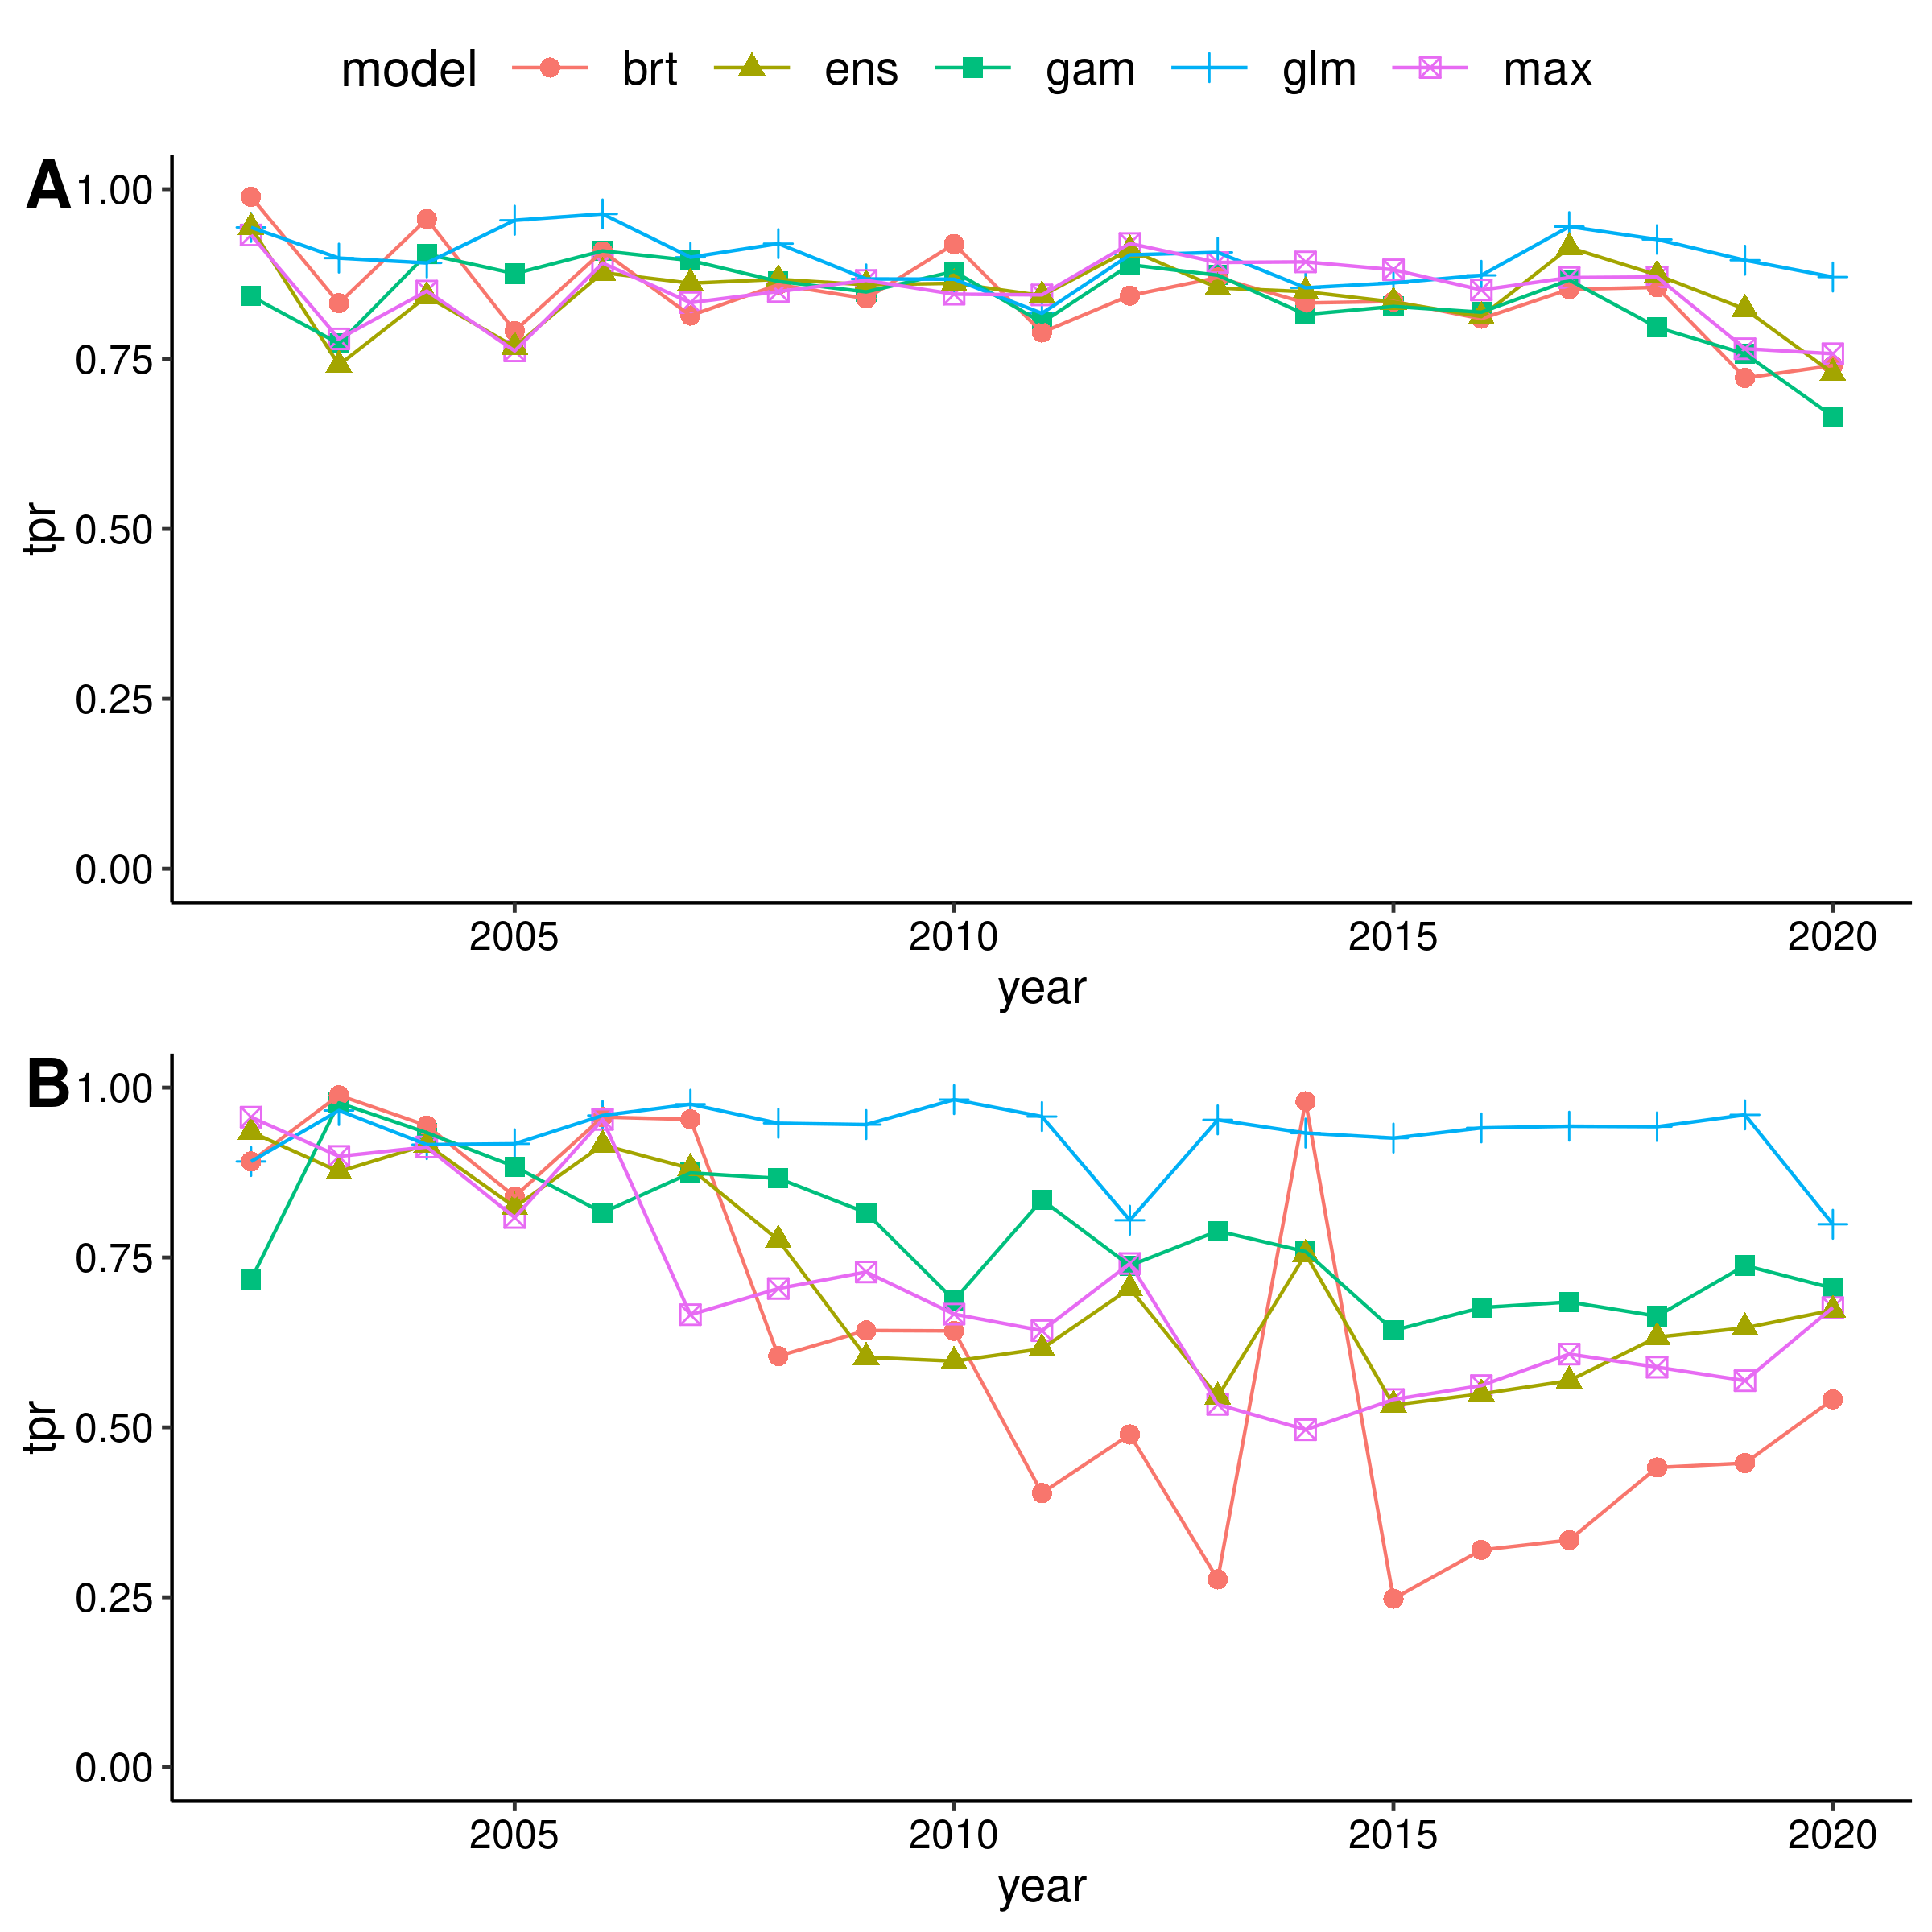
\includegraphics[width = 0.9\linewidth]{"../../R/figures/modelling-res.png"}
    \caption{\label{fig:modelling_res} SDM predictive performance over time. Subfigure A shows the performance of models created with invasive data up to the year in question in predicting the following year. Subfigure B shows the performance of models created with all the native data in predicting the year in question.}
\end{figure}

The difference in performance between the invaded and native range models is apparent, with the invaded range models achieving a higher sensitivity on average.
Surprisingly, the invasive data models already perform very well in the first years and continue to do so for all further years.
The native models vary more in their predictive performance, starting off with a sensitivity similar to that of the invaded range models, then becoming quite chaotic in performance in the years between 2008 and 2015.
After 2015, performance improves again, reaching levels close to, but still below the initial performance and that of the final invaded range models.
It is notable, that the GLM almost always performs the best out of all native models.
The model ensemble performed at least better than 50 \% of models used to build the ensemble for almost all years.

Trying to correlate the performance of each model individually to the trend in data amount or the niche stability value lead to statistically insignificant results for all models (Table \ref{tab:mod_cor_res}).

\begin{table}[H]
    \centering
    \caption{\label{tab:mod_cor_res} Results when correlating model sensitivity to either niche stability or amount of data.}
    \begin{tabular}{>{\bfseries}l r*{5}{ c}}
        \csvreader[no head, column count = 6, late after line = \\]{tab-mod-cor-res.csv}{}{\csvlinetotablerow}
    \end{tabular}
\end{table}

In the end, one can look at the model predictions for the year 2022 and compare them to the observed presences of that year (Fig. \ref{fig:mod_pred}).

\begin{figure}[H]
    \centering
    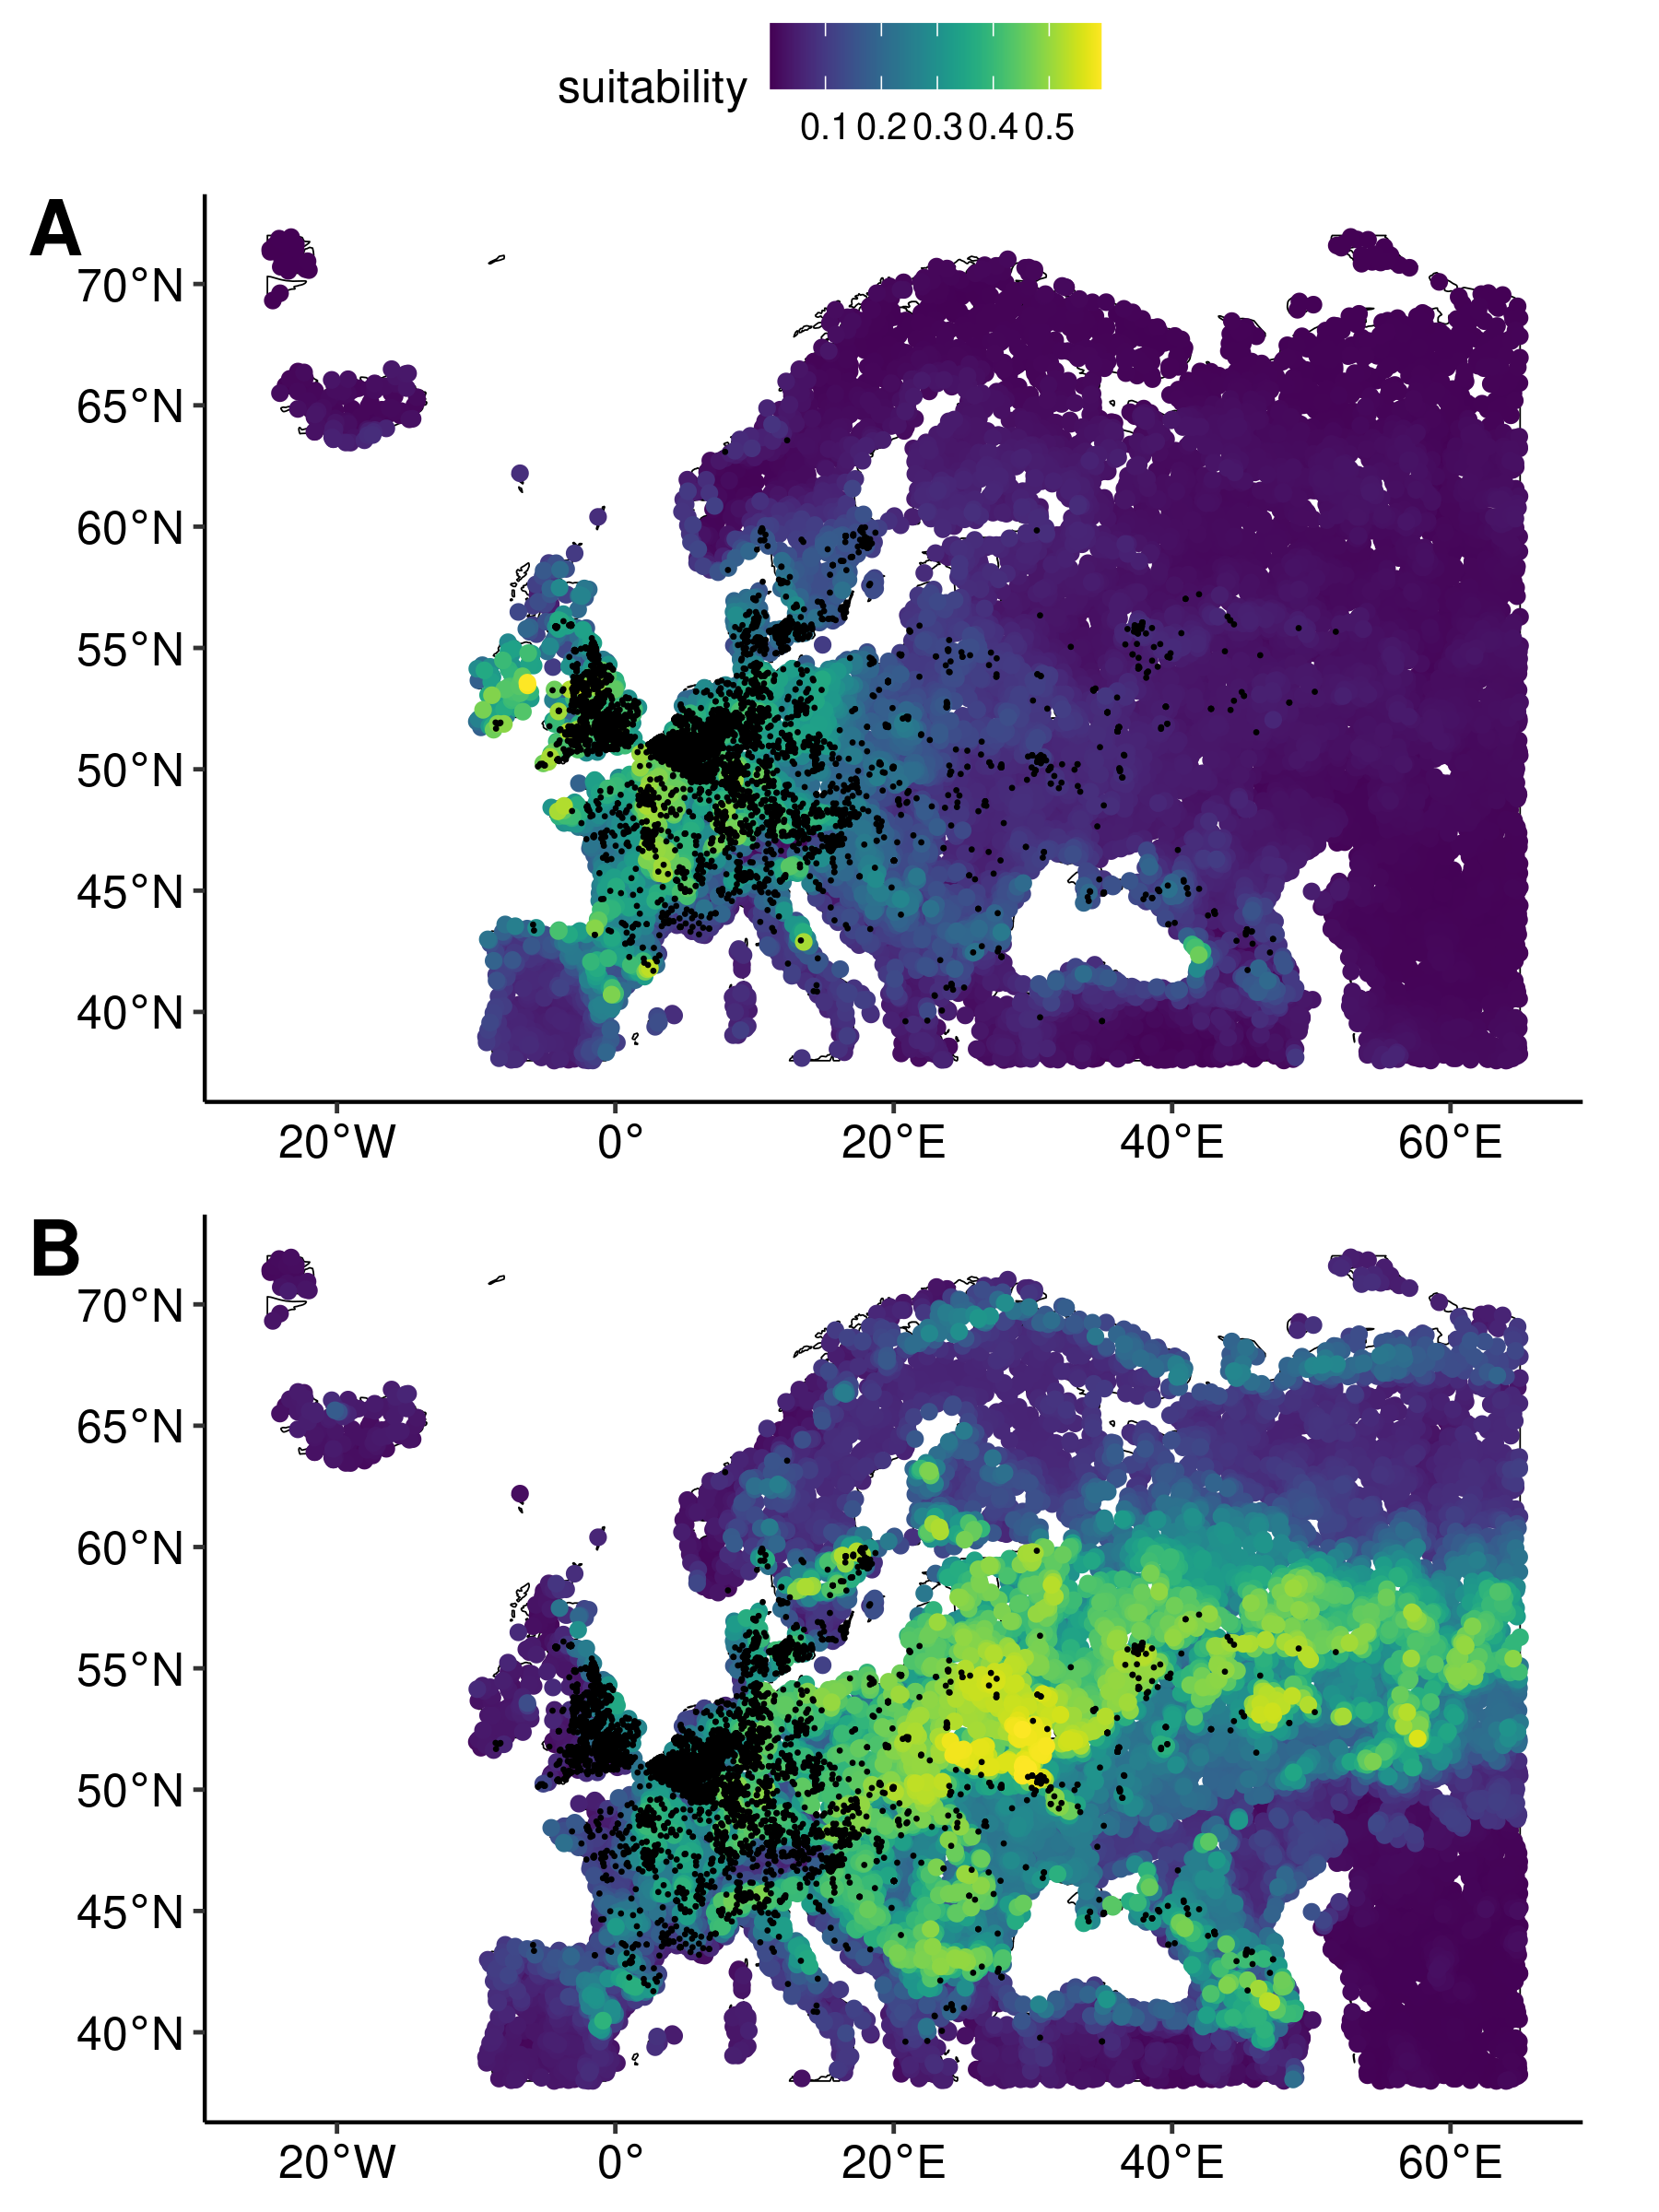
\includegraphics[width = 0.71\linewidth]{"../../R/figures/2022-mod-pred.png"}
    \caption{\label{fig:mod_pred} Predictions of the invaded (A) and native data (B) ensemble models for the suitability of \gls{harm} in 2022. Suitability shown as colour, black dots indicating presences observed in 2022.}
\end{figure}

The ensemble from the invaded range proves to be more accurate in predicting the presences of 2022, although being rather conservative in its predictions. The native ensemble predicts a much wider range in comparison, reaching much further to the east.


\newpage
\section{Discussion} \label{sec:discussion}
Using a time series of a well monitored species, it was possible to probe into the change in SDM performance over time.
It was shown that all used SDMs consistently performed very well in predicting \gls{harm} presences of the following year, when trained only on data from the invaded range in Europe.

The better performance of the invaded range models in comparison to the native models is supported by the results of niche analysis, showing that the native and invaded niche differ significantly from each other.
It has already been shown that the genetic strains of \gls{harm} present in Europe have been strongly influenced by American control strains \autocite{lombaert2010harmoniabridgehead}, so a model using American data might also prove insightful.

The consistent performance of all invaded range models might be explained in part by the rather consistent niche stability, though also in years with significant niche expansion (early years) the models are able to perform well (also see Supplementary Fig. \ref{fig:all_mod_preds} for a yearly visualization of model spatial predictions).
This could also imply that SDMs are able to perform well in environments without total niche conservatism, but the data shown in this thesis is not sufficient to make this claim.
The lack of impact of data amount on model performance suggests that the data quality of the first models was already sufficient to create good models and was not altered by the following years.
The native, as well as the invaded range ensemble predict ranges very similar to a study from 2012 \autocite{bidinger2012harmSDMglobalMaxent}, which speaks for the modelling process of this thesis.
Agreement between predictions from 2012 and models created with more recent data also supports the result of niche conservatism over this time period.

The use of sensitivity as a measure for model performance is not ideal, but was chosen instead of i.e. the True Skill Statistic due to better interpretability in the context of an invasive species.
Due to the invasive dispersal of \gls{harm} in geographical space over the years, the True Skill Statistic will for example be affected by old absences from previous years lying in areas which the species has now reached. These past absences will then be predicted as false positives.
In this way, especially absences in the area of the starting range will have a large negative impact on performance due to large numbers of false positives.
This is additionally amplified in the case of this study with the chosen bias correction (\autoref{ssec:datapreparation}), which adds pseudo-absences in areas with very high amounts of presences.
Only using sensitivity removes this issue by only looking at the amount of presences correctly classified as such.
This comes at the price of not having any measure of how well the model is able to really discriminate, making sensitivity miss issues like overprediction of suitability.
In general, there have been numerous performance metrics proposed and evaluated in order to deal with additional concerns like influences of prevalence or correct treatment of pseudo-absences compared to true sampled absences \autocite{leroy2018TSSissues, konowalik2021SDMmetrics}.
It might also be interesting to look into the period of niche expansion of \gls{harm} in more detail, for example with a monthly resolution, since data might be sufficient.

In the specific case of \gls{harm}, SDMs can definitely be used to model the current potential niche in Europe, implied by the very good performance of SDMs as shown in this case study.
The niche analysis results suggest that \gls{harm} has reached the invasion stage of ``Spread'' for quite some time already, having established a stable, occupiable niche in Europe.
Due to this, it would be more useful to also take dispersal into account in future models, since the dominating limitations of further spread will be strongly related to its dispersal ability.

While currently, \gls{harm} is not listed as a ``Species of Union Concern'' by the EU \autocite{EU2020speciesofunionconcern}, new research still keeps showing negative impacts on native environments, especially on native ladybird species \autocite{brown2022harmimpactigp}.
\gls{harm} has been indicated to have 15 other aphidophagous species as intraguild prey \autocite{lucas2007axyridisintra}.
A long term study over 11 years showed a strong negative impact of \gls{harm} on the proportion of native ladybird species in England \autocite{brown2018harmlongterm}.
\gls{harm} has also been shown to dominate ecosystems in other European countries since establishment, significantly altering local community structures \autocite{masetti2018harmitaly, honek2019harmczech}.
Further impacts of \gls{harm} remain subject of future studies.

The results of this study support the possibility for SDMs to support future endeavours to quantify the impact of \gls{harm} on native species, enhancing sampling strategies and potential spatial correlations of impact severity.

\clearpage
\section{Conclusion} \label{sec:conclusion}
The results of this thesis show that SDMs can be a strong tool in predicting the potential niche of an invasive species, even for cases of not completely static niches.
Ensembles proved to be a good way to combine different model predictions, resulting in predictions consistent with previous studies.
Using additional niche analyses provides valuable context to interpret model performance and gives additional insight into the establishment process of \gls{harm}.
It has been shown that the process used in this thesis can generate new insight into the dynamics and relations at play when dealing with invasive species and predicting their potential impact, with more interesting areas to research further.
In the specific case of \gls{harm}, this thesis shows possible future potential for SDM application in research concerning the future impact of this invasive species.


\section{Acknowledgements} \label{sec:acknowledgements}
This thesis would not have been possible in this form without the huge amount of freedom given by my main supervisor Lauren Talluto.
I was able to just try out my ideas on my own accord, which is something I value highly.
My twin brother Emanuel gave me a lot of advice on good coding practice, which helped me a lot.
I also want to thank all my friends and other relatives, who just listened to me rambling about how cool (or sometimes nerve-wracking) my progress was, even if they only understood half of it.

\newpage
\printbibliography[]


\newpage
\appendix

\newgeometry{lmargin = 3cm, rmargin = 3cm, tmargin=2cm, bmargin=2cm}
\section{Visualization of cleaned vs raw dataset}

\begin{figure}[!h]
    \centering
    \includegraphics[width = 0.8\linewidth]{"../../R/figures/raw-vs-cleaned-glob.png"}
    \caption{\label{fig:raw_vs_cleaned_glob} Visualization of the cleaned dataset for \gls{harm} in comparison to the total raw dataset. The red and green boxes show the used extents for Europe and the native range respectively, red and green points show the cleaned presence points in their respective extents, while blue points show all points of the raw dataset.}
\end{figure}



\section{Niche analysis}

\begin{figure}[!h]
    \centering
    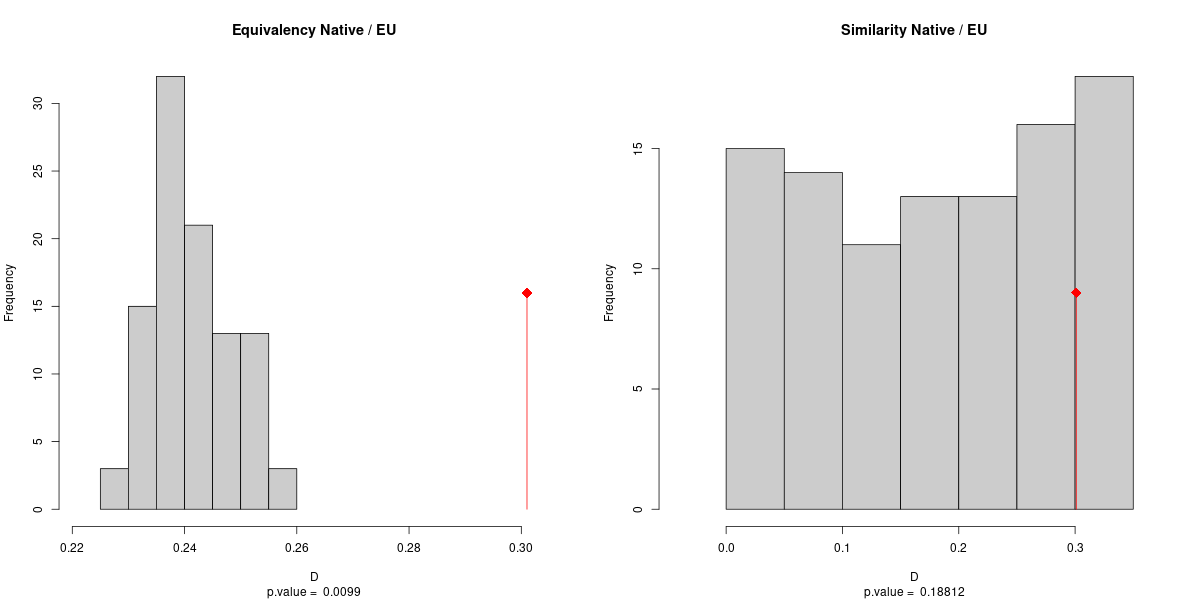
\includegraphics[width = 0.9\linewidth]{"../../R/figures/as-eu-tot-eq-sim.png"}
    \caption{\label{fig:as_eu_eq_sim} Results of the niche equivalency (left) and niche similarity (right) test comparing the native and invaded niche of \gls{harm}. Histograms of the simulated niche overlaps, the observed overlap shown as a red bar with a diamond.}
\end{figure}

\begin{figure}[!h]
    \centering
    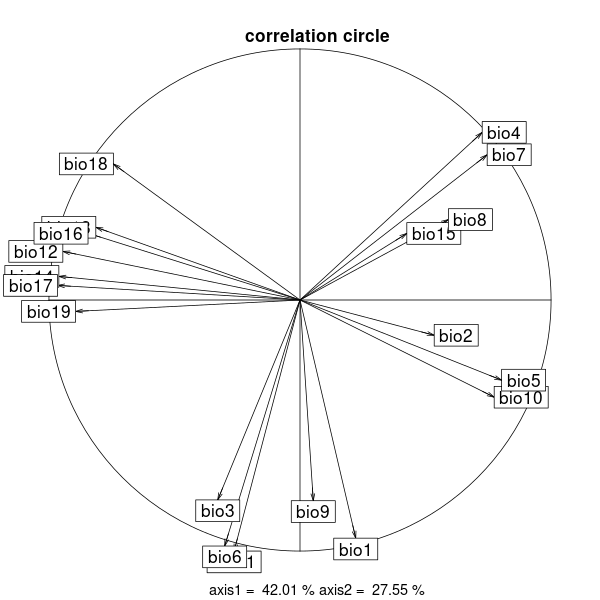
\includegraphics[width = 0.68\linewidth]{"../../R/figures/eu-years-pca.png"}
    \caption{\label{fig:eu_years_pca} Component contributions for the PCA used to conduct the niche analyses comparing each year of the invaded niche to its  following year. For detail on the bioclim variables, see (Supplementary Table \ref{tab:bioclim}).}
\end{figure}

\clearpage
\begin{table}[!h]
    \centering
    \caption{\label{tab:bioclim} Explanation of the bioclim variables (from CHELSA 2.x technical specifications).}
    \begin{tabular}{l l}
        \textbf{Variable} & \textbf{Explanation}
        \csvreader[head to column names]{tab-CHELSA-bioclim-expl.csv}{}{
        \\ \shortname & \longname
        }
    \end{tabular}
\end{table}


\clearpage
\section{Species distribution modelling}

\begin{table}[!h]
    \centering
    \caption{\label{tab:lc_contrib} Table showing PCA contributions for each Copernicus land cover class, Copernicus land cover class explanation in (Supplementary Table \ref{tab:Cop_lcc}). The last row shows the percent of total variance explained by the respective PCA axis.}
    \centerline{
        \begin{tabular}{r r*{7}{S[table-format = 1.2e2, table-align-text-pre = false, table-space-text-pre = lc]}}
            \csvreader[no head, column count = 8, late after line = \\]{tab-lc-contrib.csv}{}{\csvlinetotablerow}
        \end{tabular}
    }
\end{table}

\begin{table}[!h]
    \centering
    \caption{\label{tab:Cop_lcc} Explanation of the Copernicus land cover classes (from dataset legend).}
    \begin{tabular}{r l}
        \csvreader[no head, column count = 2, late after line = \\]{tab-Cop-lcc.csv}{}{\csvlinetotablerow}
    \end{tabular}
\end{table}

\clearpage
\begin{table}[!h]
    \centering
    \caption{\label{tab:mod_ths} Thresholds used to predict the models for the given years (inv = invaded range model (of the previous year), nat = native range model).}
    \centerline{
        \begin{tabular}{r*{11}{c}}
            \csvreader[no head, column count = 11, late after line = \\]{tab-mod-ths.csv}{}{\csvlinetotablerow}
        \end{tabular}
    }
\end{table}

\clearpage
\section{Model predictions}
\begin{figure}[!h]
    \caption{\label{fig:all_mod_preds} Predictions of each invaded range ensemble model for the year 2022, points in black showing the occurrences of the respective year, so i.e. in 2003 model it shows the occurrences of 2003, but the suitability prediction for 2022.}
    \centerline{
        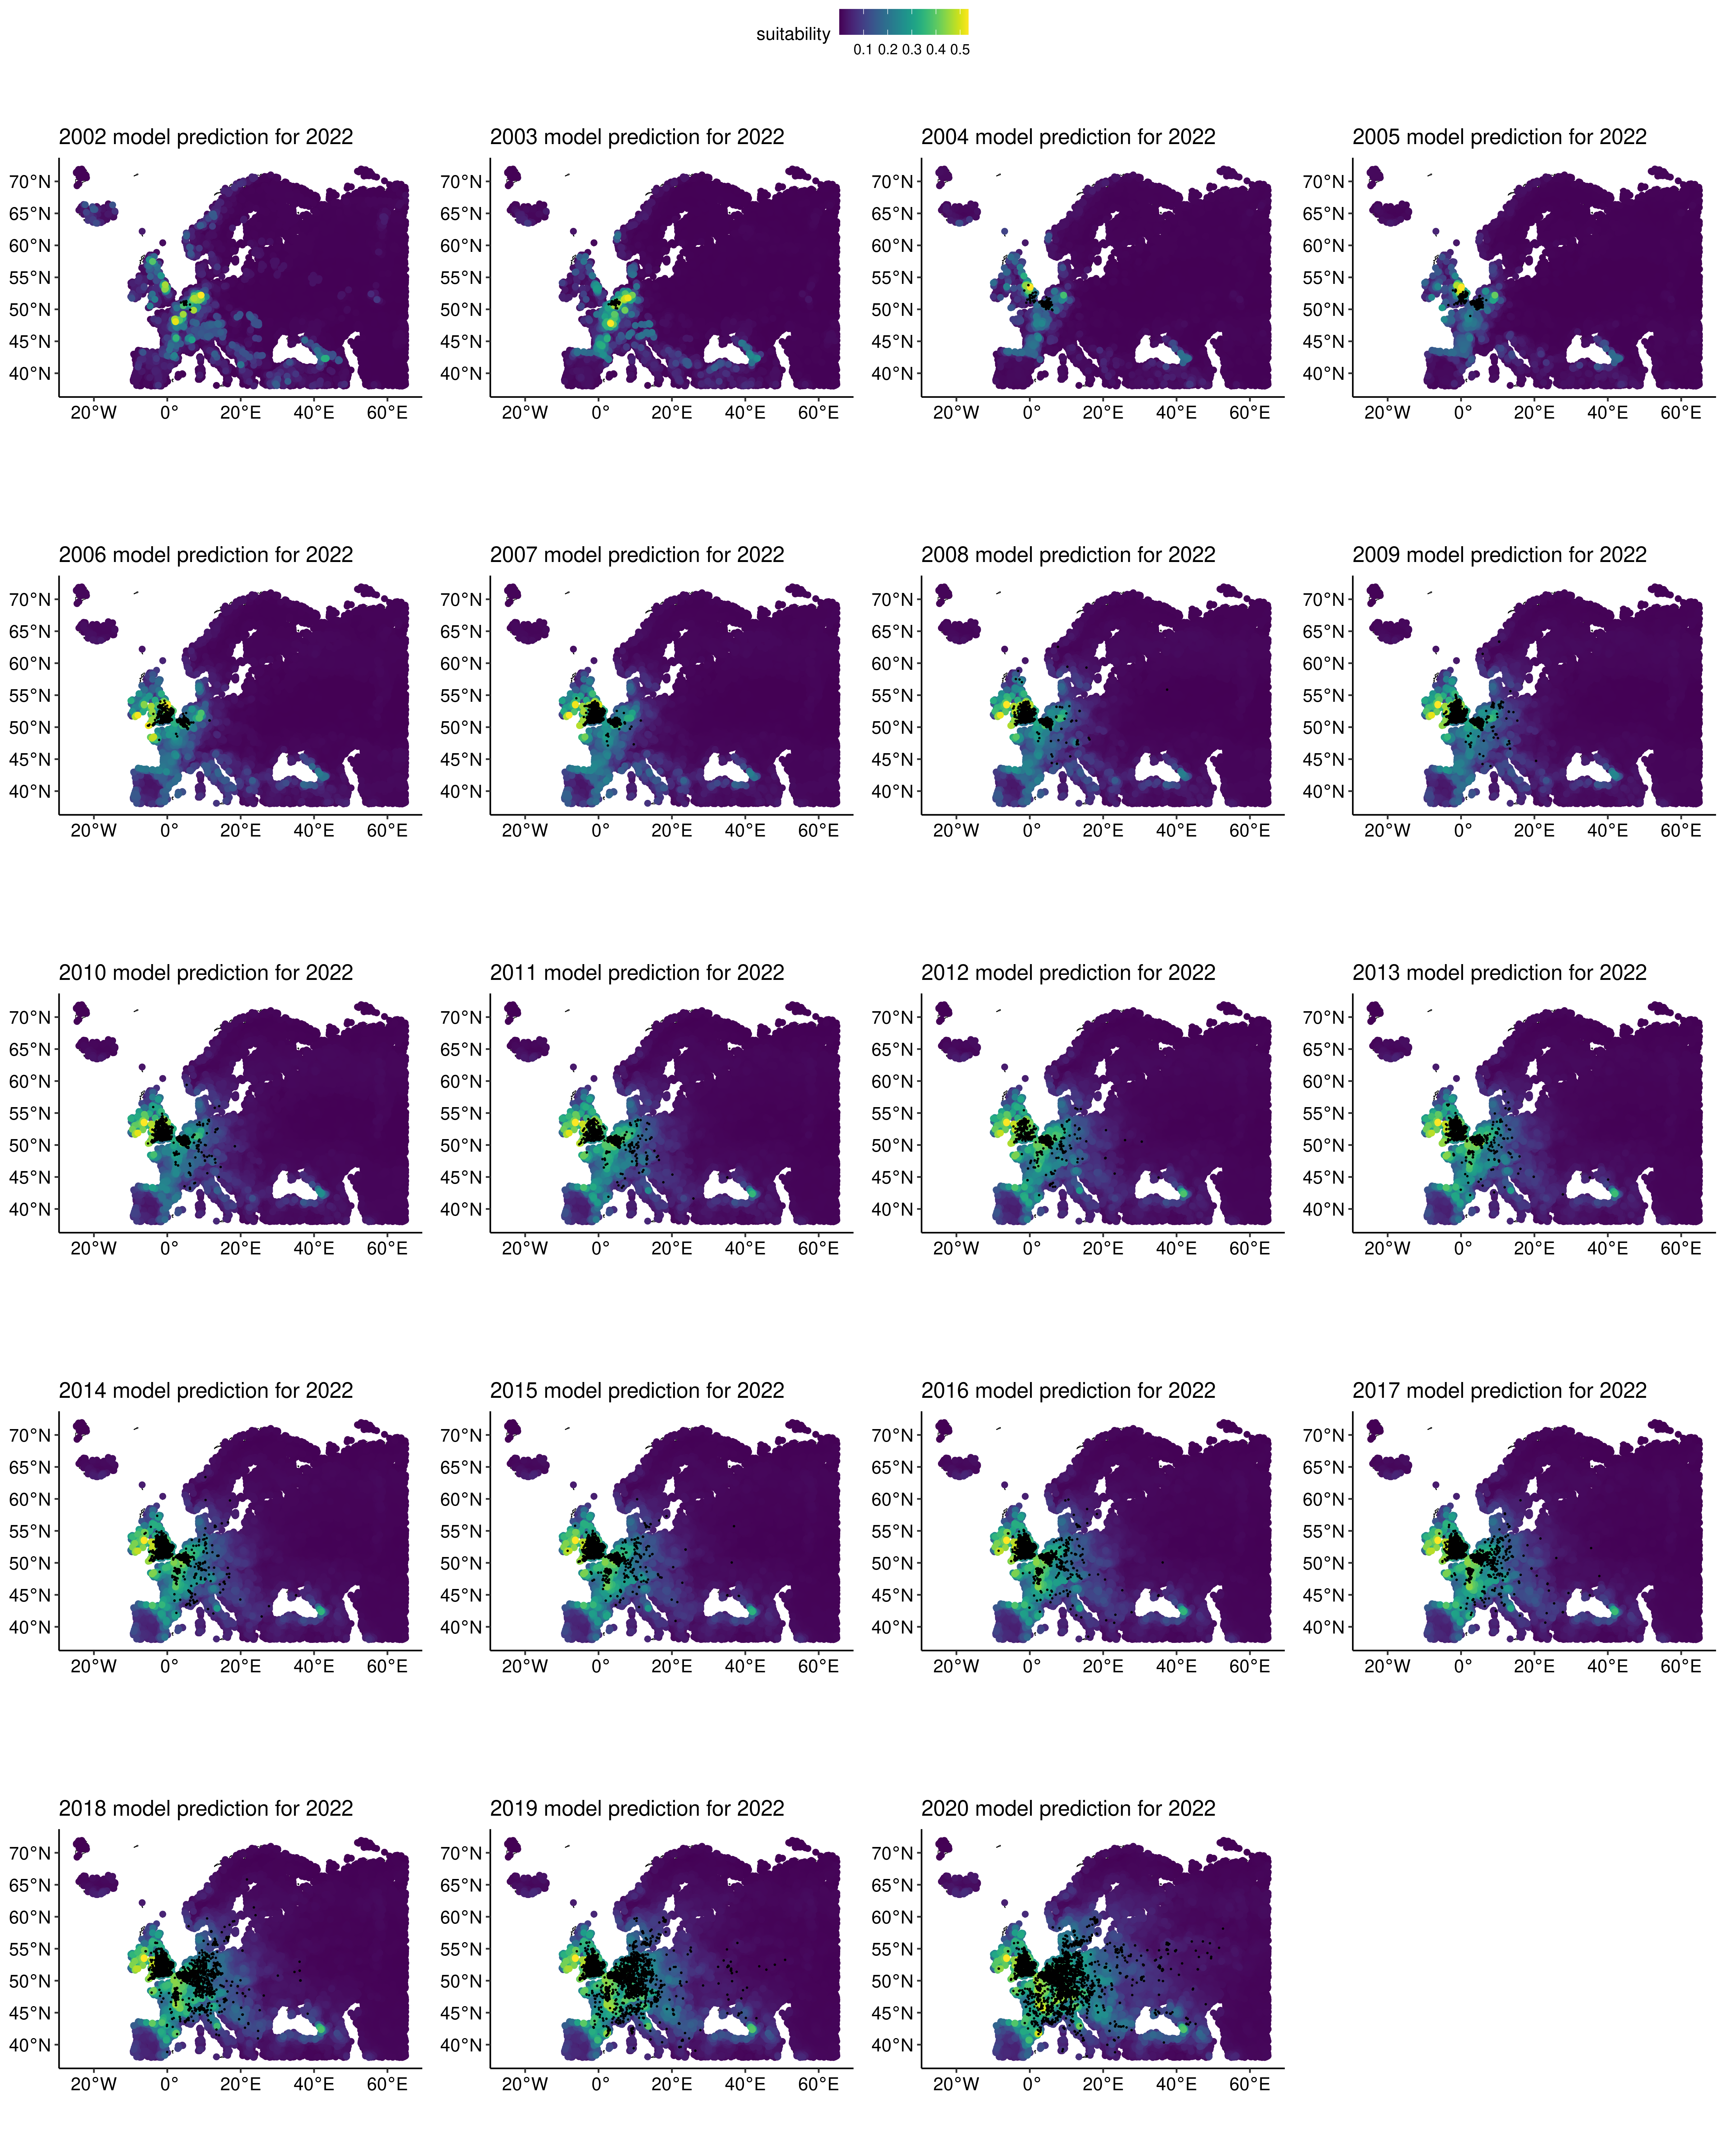
\includegraphics[width = 0.85\paperwidth, height = 0.6\paperheight]{"../../R/figures/2003to2021-mod-pred.png"}
    }
\end{figure}

\section{Model response curves} \label{sec:response_curves}

Prediction plots of all model variables, showing histograms of the training data for each separate variable (absences and presences separated) in comparison to the suitabilities in the data range, predicted by the calculated models, plotted as response curves.

\begin{figure}[!ht]
    \caption*{Native model response curves}
    \centerline{
        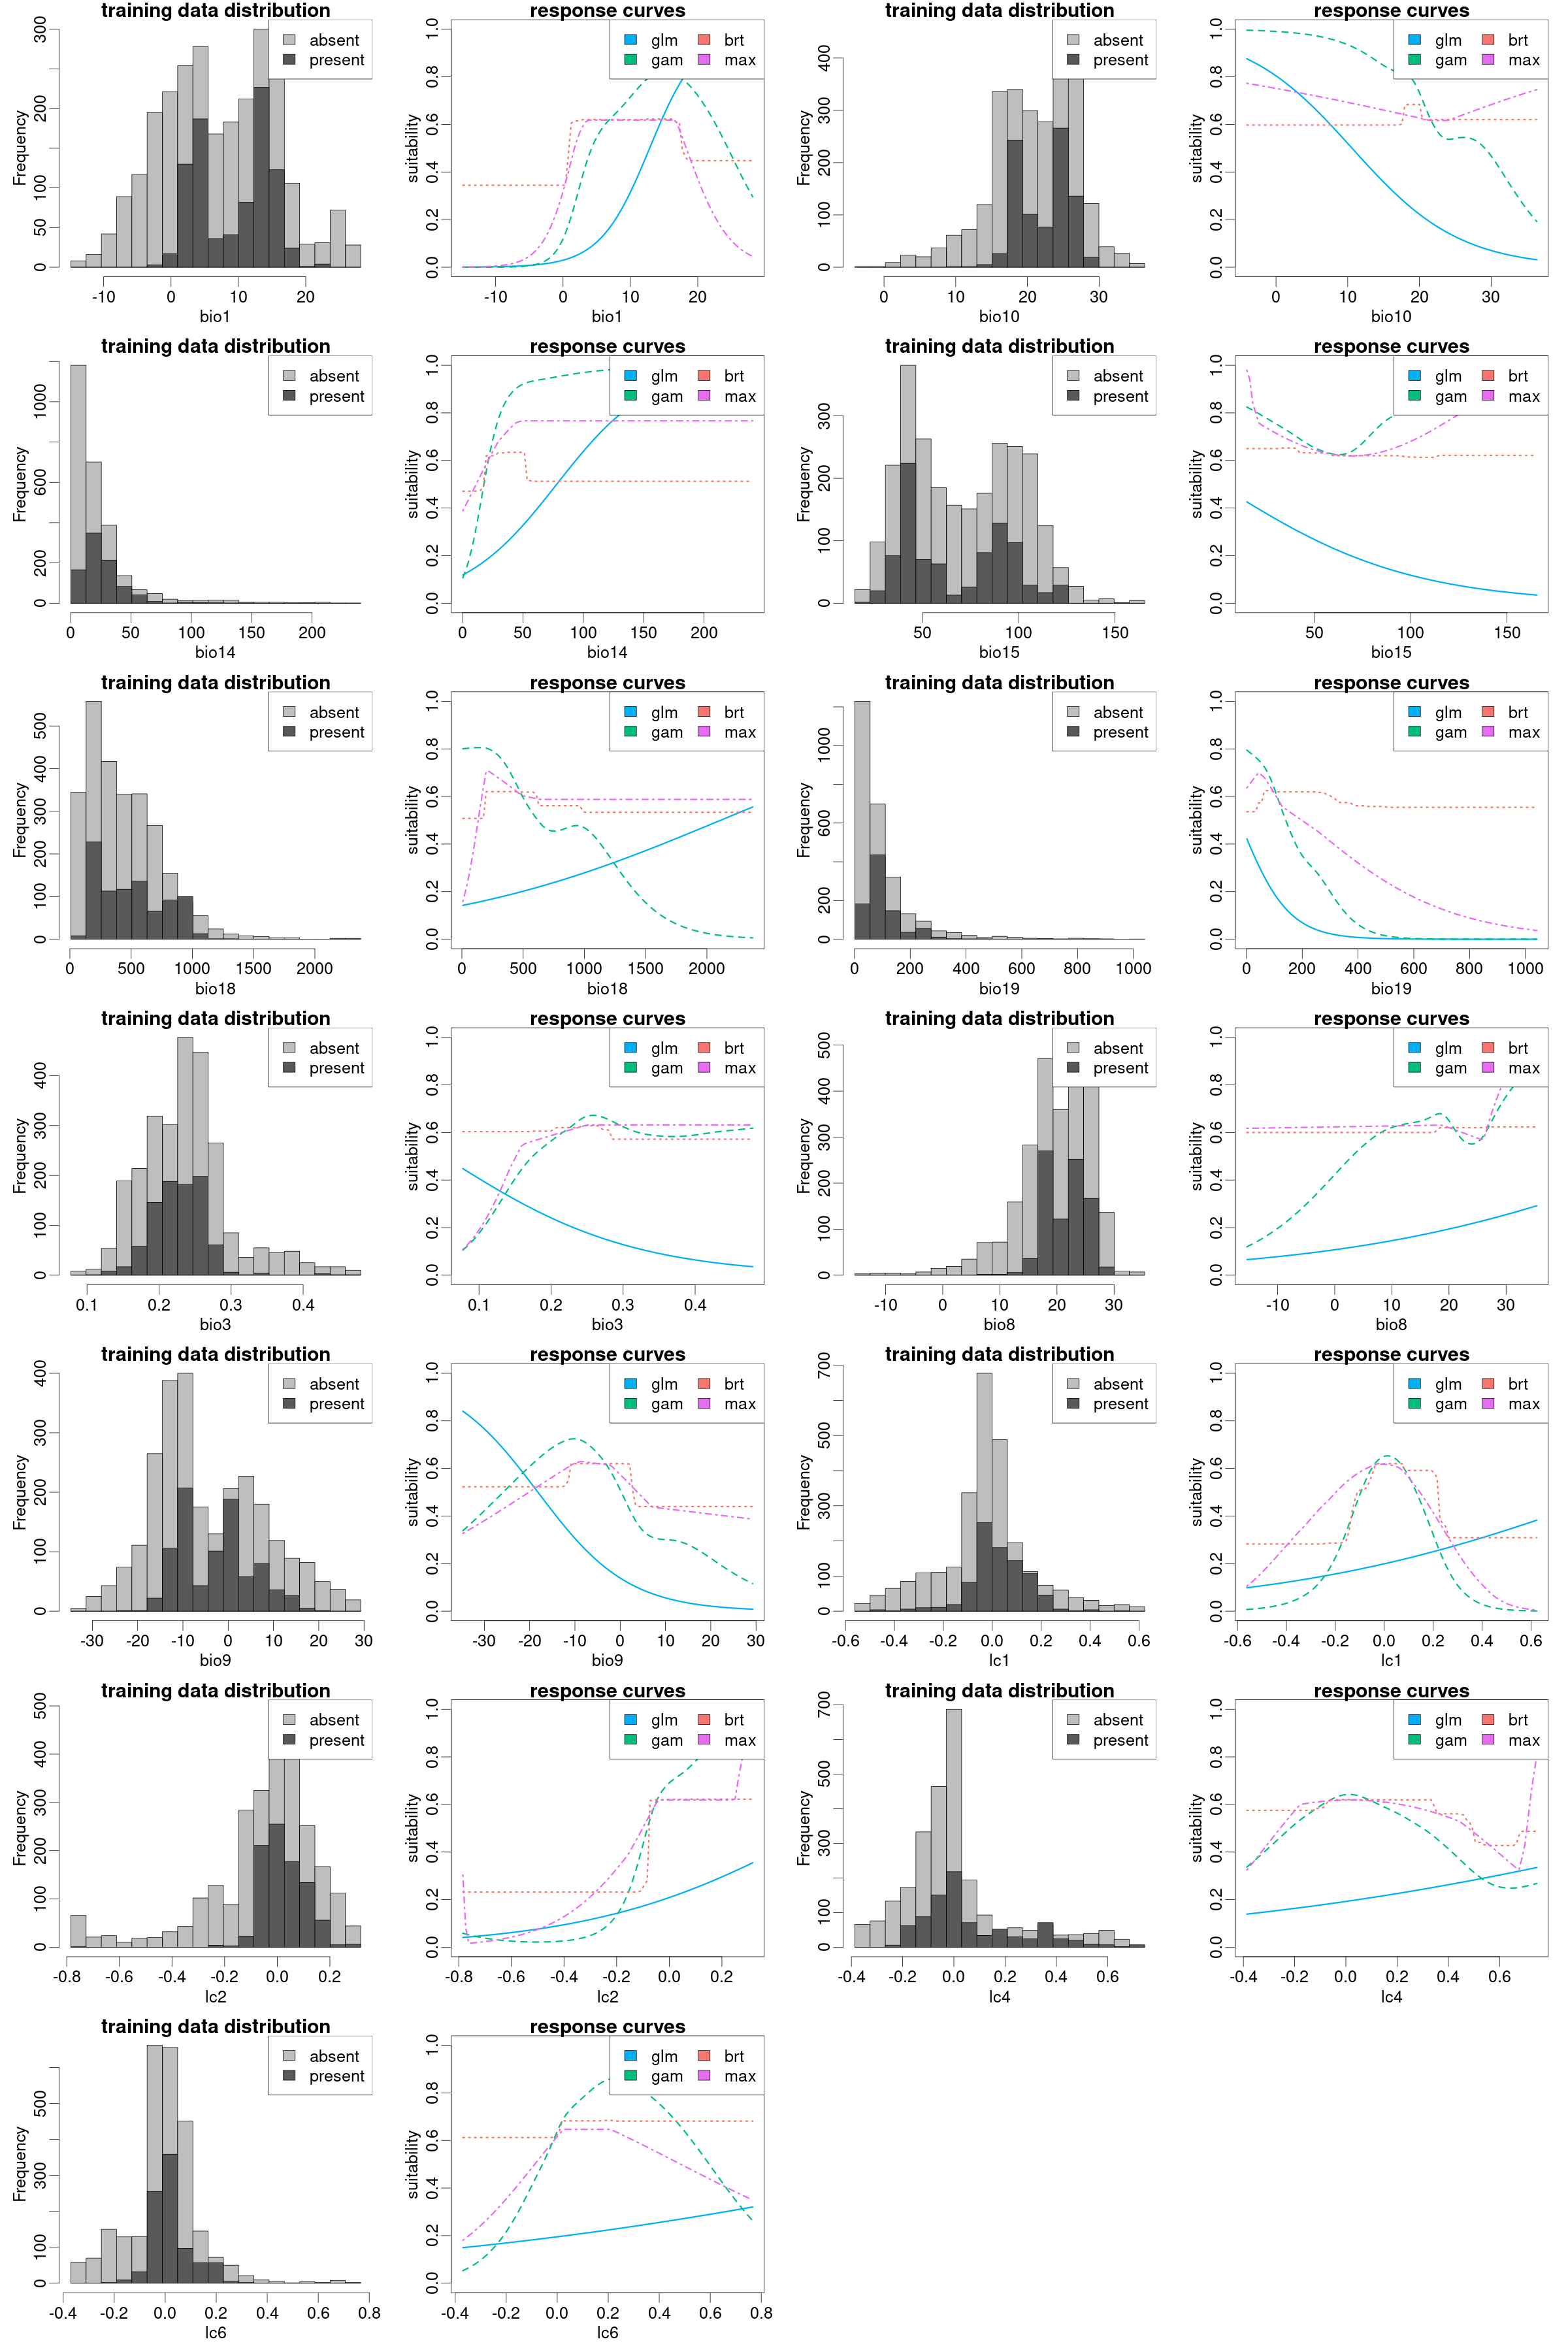
\includegraphics[width = 0.9\paperwidth, height = 0.83\paperheight]{"../../R/plots/response_curves/native_mod_resp.png"}
    }
\end{figure}



\foreach \y in {2002,...,2020}{
        \begin{figure}[!ht]
            \caption*{\y \ model response curves}
            \centerline{
                \includegraphics[width = 0.9\paperwidth, height = 0.83\paperheight]{"../../R/plots/response_curves/\y_mod_resp.png"}
            }
        \end{figure}
    }

\end{document}